% AEC Interpreter — research-paper assembly (standard structure:
% Intro w/ related work + contributions → System Design → Evaluation → Discussion → Conclusion).
% Structure follows the draft in "AEC Interpreter - org.md" §Draft structure.
% Compile:  pdflatex main && bibtex main && pdflatex main && pdflatex main   (see Makefile).
\documentclass[11pt]{article}

\PassOptionsToPackage{hyphens}{url}
\usepackage[utf8]{inputenc}
\usepackage[T1]{fontenc}
\usepackage{lmodern}
\usepackage[margin=1in]{geometry}
\usepackage{graphicx}
\usepackage{booktabs}
\usepackage{amsmath}
\usepackage{amssymb}
\usepackage[protrusion=true,expansion=true]{microtype}
\usepackage[numbers,sort&compress]{natbib}
\usepackage{xcolor}
\usepackage[colorlinks=true,linkcolor=black,citecolor=blue,urlcolor=blue]{hyperref}

\graphicspath{{figures/}}

% Section cross-reference shorthand used in the prose.
\newcommand{\secref}[1]{\S\ref{#1}}

\title{\bfseries AEC Interpreter: Cross-Modal Alignment and\\
Ontology-Driven Retrieval for Site-to-BIM Element Grounding}
\author{Chia Hui Yen\\
\small Carnegie Mellon University\\
\small \texttt{huiyenc@andrew.cmu.edu}}
\date{2026}

\begin{document}

\maketitle

\begin{abstract}
Architecture, Engineering, and Construction workflows still depend on people translating
egocentric site evidence --- photographs, marked plans, and short notes --- into allocentric BIM
records. Before an AI system can reason about status, schedule, or corrective action, it must answer
a more basic spatial question: \emph{which exact model element is this?} We introduce a
neuro-symbolic image-to-BIM grounding method that maps a construction-site photograph and
natural-language note to a \emph{unique} IFC element GUID using only the BIM model itself for
supervision, with no real on-site labels. The task is hard because many candidate elements are
\emph{visually identical}, the target identity lives in \emph{graph} space while the evidence lives
in \emph{image} space, and a cold-start deployment has no paired site-image training set. Our method
recovers a \textbf{type-conditional spatial address} --- a class-specific relational key, such as an
opening's ordinal position-slot or a wall's connectivity fingerprint, that is computable from the
raw IFC model and recoverable from image/plan evidence. A vocabulary-constrained neural layer reads
coarse semantics; deterministic visual specialists recover discriminating address fields; and a
symbolic executor consumes a per-field \texttt{\{value, confidence, source\}} contract through
recall-safe reranking and selective prediction. Supplied at an oracle level, the address lifts pool
Top-1 from 4.9\% to \textbf{78.5\%} at zero recall cost; a single realizable position-slot extractor
lifts the addressable subset from a 6.6\% floor to \textbf{67.6\%}; its confidence passes an ECE
calibration gate (AUROC 0.80); and deferring the least-confident fifth raises answered-set Top-1 to
\textbf{80.6\%}. The result is an auditable spatial multimodal grounding layer for AEC: ontology is
the guardrail, topology is the discriminator, and the system knows when to abstain.

\end{abstract}

\noindent\textbf{Keywords:} AEC, spatial intelligence, neuro-symbolic grounding, IFC, vision-language models

\section{Introduction}
\label{sec:intro}

\subsection{Motivation: bridging physical site evidence and digital truth}

AEC coordination moves constantly between two incompatible views of the same building. On site,
evidence is egocentric and fragmented: a phone photograph, a marked floorplan crop, a short chat
message from a front-line worker. In the project record, truth is allocentric and structured: a BIM
model, IFC element types, topology, and GUIDs. The traceability gap is the missing translation between
these two views. A coordinator does not merely need to know that an image contains \emph{a window};
they need to know which of the many near-identical windows in the BIM cloud should receive the issue,
handoff record, or BCF link. Before an AI system can answer higher-level AEC questions --- what
happened, who is responsible, what action should follow --- it must solve the foundational grounding
question: \emph{where exactly is it in the model?}

The setting is deliberately cold-start. A construction or facilities team has a complete IFC/BIM
model but no history of labelled site imagery; on day one they want to point a phone at an element,
add a short note, and be told \emph{which} modelled element it is. The final step is a selection from
a retrieved candidate pool in which the ground truth is present (median 76, in-pool 100\%), so the
difficulty is not retrieval but \textbf{discrimination among visually identical siblings}, in a regime
with no paired supervision to learn that discrimination from. The natural baseline --- fine-tune a
multimodal reranker to score the pool end-to-end --- is exactly the configuration that plateaus: it
reaches Top-1 6.7\% with the answer already in the pool, because the signal that separates two
identical windows is not in either window's pixels but in the building's relational structure, which a
black-box matcher must reconstruct internally and unreliably (we develop this design rationale in
\secref{sec:rationale}~\citep{sutton2019bitter}).

\subsection{Research questions}

This paper makes one contribution --- an \textbf{ontology-grounded, topology-derived spatial
address} and the calibrated routing that makes it usable. Ontology supplies the floor and the
guardrail: the vocabulary, storey, class, and schema-compliant execution boundary that prevent
hallucinated element IDs. Topology supplies the discriminator: the local relational structure that
separates visually identical siblings. The contribution is developed through three research
questions:

\begin{itemize}
  \item \textbf{RQ1 --- Representation (\secref{sec:eval-oracle}).} \emph{What is the minimal sufficient
  spatial address?} We show it is \textbf{type-conditional}: a coarse ontological prefix (storey +
  class) that is necessary but saturated, completed by a class-specific topological body --- the
  position-slot $(i, M)$ for fillers, a connectivity fingerprint for walls. At an oracle level it
  reorders the pool from Top-1 4.9\% to \textbf{78.5\%}, with the gain partitioned by element type
  (fillers 91\%, walls 64\%).

  \item \textbf{RQ2 --- Mechanism (\secref{sec:eval-realized}).} \emph{How is a noisily-recovered address
  used without losing recall, and how much of the ceiling is realizable?} Hard filtering destroys recall,
  so the address is a \textbf{soft prior in a recall-fixed pool}; one real extractor lifts the
  addressable Top-1 from 6.6\% to \textbf{67.6\%}, its confidence passes an ECE gate (AUROC 0.80),
  and --- since reweighting a finest-grained prior is a no-op --- its payoff is \textbf{selective
  prediction}: deferring the least-confident ${\sim}20\%$ raises answered-set Top-1 to \textbf{80.6\%}
  \citep{guo2017calibration, geifman2017selective}.

  \item \textbf{RQ3 --- Architecture (\secref{sec:eval-depth}).} \emph{Where should the relational context
  live --- extracted deep at inference, or compiled into the node?} A \textbf{depth law}: deeper
  context is informationally more discriminative but its recovery collapses with depth (per-hop
  reliability $0.40 \to 0.05 \to 0$), so the realizable confusable set saturates at one hop (median
  $13 \to 8.2 \to 8.1$). The architecture therefore compiles depth into the node and extracts at
  depth $\le 1$, placing learning at the neural$\to$symbolic interface \citep{mao2019nscl}.
\end{itemize}

\subsection{Related work and positioning}
\label{sec:related}

Prior work approaches the image-to-building-model problem from two directions that do not meet in
the middle.

\paragraph{Vision-language spatial perception.} One line endows VLMs with spatial reasoning by
training on synthetic spatial-QA data; SpatialVLM demonstrates that metric and relational spatial
judgments are learnable from generated supervision \citep{chen2024spatialvlm}, and VLM-based
scene-graph extraction recovers object-relation structure from images.
% TODO [CITATION NEEDED]: the org note also names "Li et al. 2024" and "Wang et al. 2024"
% (pixels-to-graphs VLMs) — could not verify which papers these are; confirm before adding.
These systems answer in \emph{image} space --- a region, a relation, a distance --- and stop at the
image boundary: none of them names an element in a building's authoritative model.

\paragraph{LLM-driven graph retrieval.} A second line connects language models to graph stores.
Document-level GraphRAG builds its graph by LLM extraction from text \citep{edge2024graphrag}, which
is noisy in AEC because element attributes and spatial relationships are rarely verbalized;
text-to-Cypher generation hallucinates node and relationship names and requires LLM-supervised
verification scaffolding to approach reliability \citep{tiwari2024autocypher, gusarov2025graphrag}.
IFC-native systems avoid the noisy-graph problem by building on the schema directly: IFC-graph
converts the model into a queryable property graph \citep{zhu2023ifcgraph}, Graph-RAG pipelines
extract information from IFC data \citep{iranmanesh2025ifcgraphrag}, and MCP4IFC drives IFC-based
design through LLM tool calls \citep{nithyanantham2025mcp4ifc}; Text2BIM generates building models
from language \citep{du2024text2bim}. All of these, however, operate on \emph{structured or textual}
queries --- none grounds unstructured multimodal site evidence to an element.

\paragraph{Positioning.} To our knowledge, this is the first work to combine open-vocabulary
multimodal perception with IFC-native deterministic graph retrieval for \emph{element-level}
grounding in construction site workflows. Prior IFC-based systems
\citep{nithyanantham2025mcp4ifc, iranmanesh2025ifcgraphrag} operate on structured queries; prior
VLM-based spatial systems \citep{chen2024spatialvlm} lack IFC-grounded retrieval. This work bridges
the gap, placing the system in the high-determinism, multimodal-input quadrant of the landscape:
flexible vision-language perception on the input side, ontology-constrained graph execution on the
output side, with a calibrated routing layer between them. The neuro-symbolic precedent --- neural
perception feeding a symbolic executor, with learning at the interface --- is the concept-learner
line \citep{mao2019nscl}.

\subsection{Contributions}

\begin{enumerate}
  \item \textbf{A neuro-symbolic interpreter architecture} that maps unstructured multimodal AEC
  evidence (photo + note + plan) to IFC element GUIDs via a structured intermediate representation
  --- a per-field \texttt{\{value, confidence, source\}} contract --- achieving hallucination-resistant
  retrieval: the neural layer describes evidence, but only the symbolic layer names GUIDs
  (\secref{sec:design}).

  \item \textbf{A type-conditional, image-recoverable spatial address} --- the ordinal position-slot
  for openings, a connectivity fingerprint for walls --- computable from the raw IFC model with no
  human labels, that reorders the retrieved pool from Top-1 4.9\% to 78.5\% at an oracle level and
  underlies the realized 67.6\% (\secref{sec:eval-oracle}, \secref{sec:eval-realized}).

  \item \textbf{An oracle-based evaluation methodology} that decomposes retrieval failure into the
  symbolic-layer ceiling versus neural extraction quality --- demonstrating 100\% ground-truth
  retention, isolating extraction as the bottleneck, and yielding a recall-safety principle (union,
  never intersection, when combining mature and immature signals) and a measured depth law for
  relational context (\secref{sec:eval}).

  \item \textbf{An empirical analysis of where learned and deterministic components belong}: a
  per-field profile of a LoRA fine-tuned VLM showing saturation on coarse fields and failure on
  discriminating ones, motivating delegation to deterministic visual specialists with calibrated,
  selectively-predictive routing (ECE gate, defer-on-low-confidence) rather than further fine-tuning
  (\secref{sec:eval-neural}, \secref{sec:eval-realized}).
\end{enumerate}

\subsection{Scope, stated up front}

Two honesty boundaries frame every result. First, the diagnostic ceilings (RQ1, and the oracle rows
of the evaluation) assume perfect extraction; the realizable numbers come from one deterministic
extractor (the position-slot), with the wall fingerprint and remaining descriptors demonstrated at
oracle level only --- full realization is future work. Second, all measurements are on a single
synthetic project (cold-start by design); the \emph{form} of the contribution --- a type-conditional,
shallow, image-recoverable, calibrated-soft address --- is general, but the specific reliabilities are
project-specific. To keep the claim anchored beyond our own ablations, we add standard lexical and
dense retrieval baselines and a triage-effort proxy: generic retrievers plateau at Top-1 1.7\% /
Top-10 15.6--25.0\%, the realized position-slot specialist closes the filler subset to 67.6\% Top-1,
and the perfect-address ceiling reduces expected inspection effort from a median 38 candidates to 0.5.
We do not claim to beat an end-to-end matcher in the large-data limit; we claim that in the cold-start
regime we can actually measure, the structured address is what makes grounding realizable, auditable,
and transferable.

\section{System Design}
\label{sec:design}

\subsection{Design rationale: four decisions, each against a measured alternative}
\label{sec:rationale}

The architecture is best explained by the alternatives it rejects. Each key decision below names the
rejected alternative, the evidence against it, and the trade-off accepted; Figure~\ref{fig:rationale}
collects the four head-to-head measurements.

\begin{figure}[t]
  \centering
  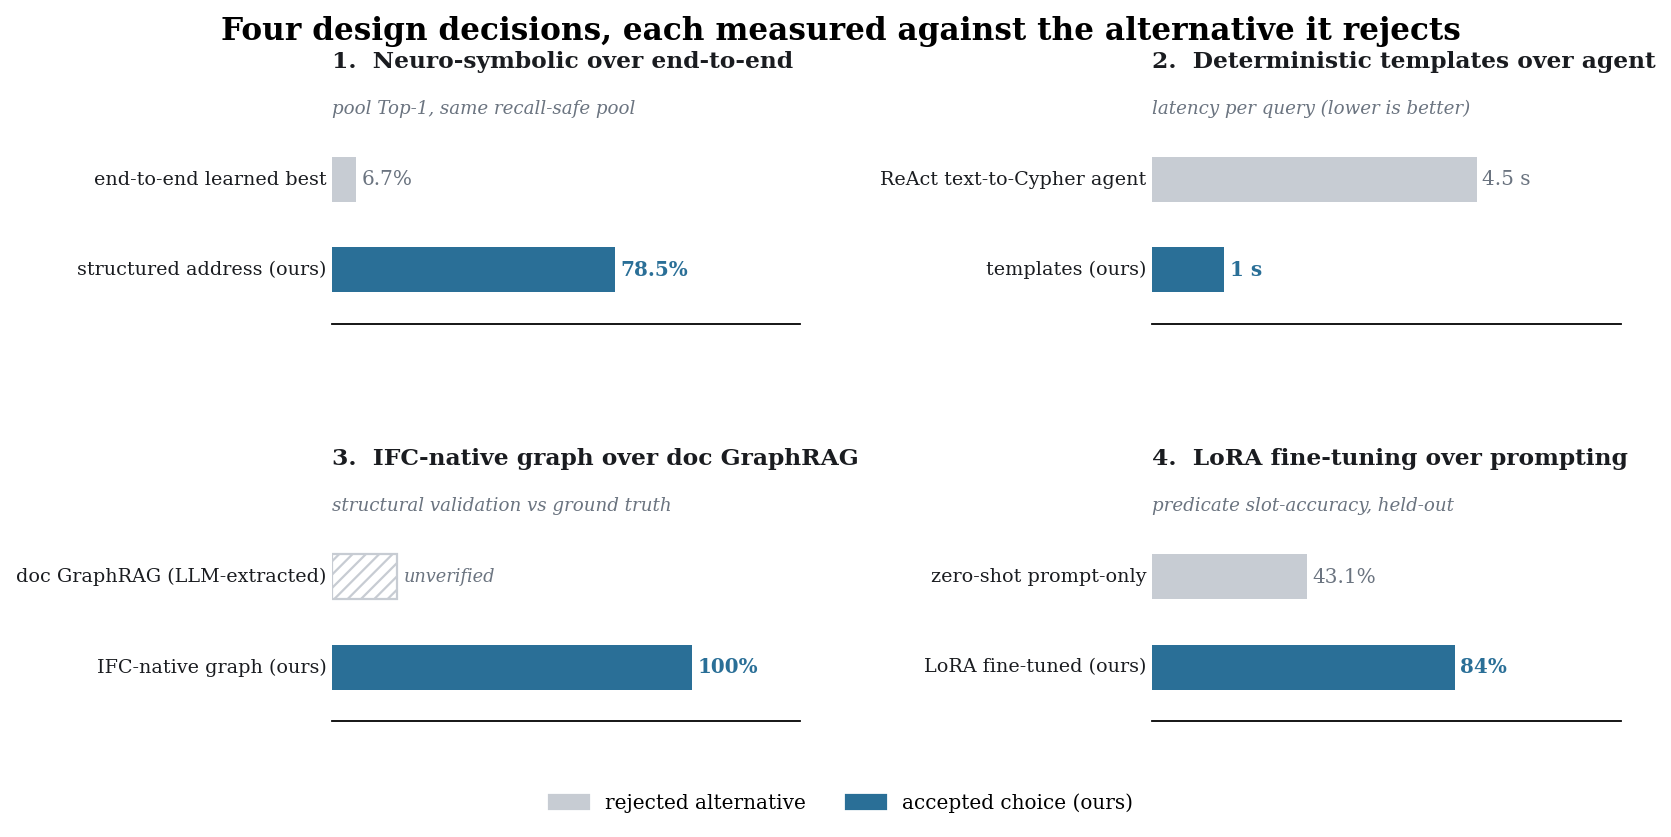
\includegraphics[width=\textwidth]{design_rationale.png}
  \caption{Four design decisions, each against the alternative it rejects, on a single measured
  quantity (grey = rejected, colour = accepted). (1)~On the same recall-safe pool, the strongest
  learned end-to-end configuration ranks the target at Top-1 6.7\% while the structured address
  reaches 78.5\%. (2)~Deterministic query templates run at ${\sim}1$\,s with 100\% syntax
  correctness and exact repeatability, versus a ${\sim}4.5$\,s ReAct text-to-Cypher agent that picks
  different tools per run. (3)~The IFC-native graph is validated against ground truth (wall
  \texttt{connection\_degree} 14/14), whereas a document-GraphRAG graph is LLM-extracted and
  unverified. (4)~LoRA fine-tuning lifts spatial-direction accuracy from ${\sim}0\%$ to 82\% (coarse
  fields 30--63\% $\to$ 100\%).}
  \label{fig:rationale}
\end{figure}

\paragraph{Why neuro-symbolic over end-to-end neural matching?} The obvious design --- train a single
cross-attention model to compare the site evidence against the candidates and rank them end-to-end
--- is, in its strongest ``bitter-lesson'' form \citep{sutton2019bitter}, the objection the design
must answer, and we answer it empirically. First, the candidates are graph nodes, not images: they
carry no photograph, and an image-space grounding result (a region in a photo or plan) does not reach
a GUID, because image space and graph space are not co-registered. The only bridge is a representation
independent of the image's coordinate frame --- a coordinate-free relational address. Second, the
discriminative signal is relational, not pixel-local: what separates two visually identical windows is
graph topology (``the third of five fillers along an external wall''), which a pixel matcher would
have to re-derive inside its own weights --- unreliably, as the classical opening-count baseline
(${\sim}27\%$) illustrates. Third, our strongest \emph{learned}
configuration plateaus on this discrimination: the fine-tuned-VLM extraction pipeline (\emph{G8}),
feeding deterministic retrieval with no within-pool reranking, reaches Top-1 6.7\% with the answer
in the pool 100\% of the time, and generic lexical/dense retrievers over the same pool reach Top-1
$\le 1.7\%$ (\secref{sec:eval-oracle}); the same pool reorders to 78.5\% when the relational address
is supplied. We do not train a dedicated end-to-end cross-attention matcher over the pool: its
inputs would be the site image against text-identical sibling candidates (the graph nodes carry no
images), so it would have to recover the same relational signal internally --- the configuration we
argue against; a zero-shot VLM reranker as the off-the-shelf upper-bound of that family is left as a
baseline to add (\secref{sec:limitations}). Finally, construction compliance requires
repeatability and audit: a scalar matching score is not auditable, not correctable, and cannot be
gated by per-field calibrated confidence. Trade-off accepted: less end-to-end flexibility, in exchange
for recall guarantees, auditability, and zero-shot transfer of the address to any IFC model.

\paragraph{Why deterministic query templates over text-to-Cypher?} LLM-generated Cypher produces
syntax errors and hallucinates node and relationship names; even dedicated systems need an
LLM-supervised generation-verification loop to approach reliability
\citep{tiwari2024autocypher, gusarov2025graphrag}. Our query patterns are enumerable (nine strategies)
and domain-specific, so a fixed template with parameter slots gives 100\% syntax correctness. The
agentic alternative was tested directly (timings from prior thesis work): a ReAct-style agent ran at
${\sim}4.5$\,s versus ${\sim}1$\,s for the constrained pipeline and chose different tool sequences for
the same input --- unacceptable where the same photo must always produce the same result. Trade-off accepted: only predefined query
patterns are covered, not arbitrary questions.

\paragraph{Why an IFC-native graph over document-level GraphRAG?} Document GraphRAG builds its graph
by LLM extraction from text \citep{edge2024graphrag} --- noisy in AEC, where element attributes and
spatial relationships are rarely verbalized. Our graph is compiled from the IFC schema directly
\citep{zhu2023ifcgraph, buildingsmart2024ifc4x3}, so the graph itself is zero-error ground truth.
Trade-off accepted: the system requires a project IFC file and cannot answer questions about things
absent from the model.

\paragraph{Why fine-tuning over prompting-only?} Few-shot prompting is stateless --- it cannot improve
over a project's lifecycle. LoRA fine-tuning accumulates field feedback as supervised examples for
periodic retraining, and runs locally at ${\sim}1$\,s with no per-call API cost versus 3--5\,s for a
prompted frontier model. Trade-off accepted: a synthetic data pipeline and retraining infrastructure
are required (\secref{sec:synth}).

\subsection{Architecture overview}
\label{sec:arch}

The pipeline has five stages: multimodal input (photo + note + plan crop) $\to$ neural extraction into
a typed record $\to$ a structured constraint contract $\to$ deterministic query compilation against the
IFC graph $\to$ a ranked GUID shortlist or an explicit deferral. Figure~\ref{fig:pipeline} traces a
single case through the spine, with the confidence-routing path --- from the extractors'
\texttt{\{value, confidence, source\}} records to the answer/defer gate --- highlighted; that path is
the system's determinism$\leftrightarrow$adaptivity mechanism. The evidence flow is intentionally
ordered from raw observation to auditable execution: a vocabulary-constrained VLM reads the coarse
semantic prefix; deterministic specialists recover the fields the VLM does not carry reliably; the IFC
graph supplies the legal candidate universe and precomputed topology; and the routing layer decides
whether the recovered address is confident enough to answer or should surface a candidate set for
human verification. This ordering is the hallucination control: \textbf{the neural layer describes
evidence, but the symbolic layer alone names GUIDs.}

\begin{figure}[ht]
  \centering
  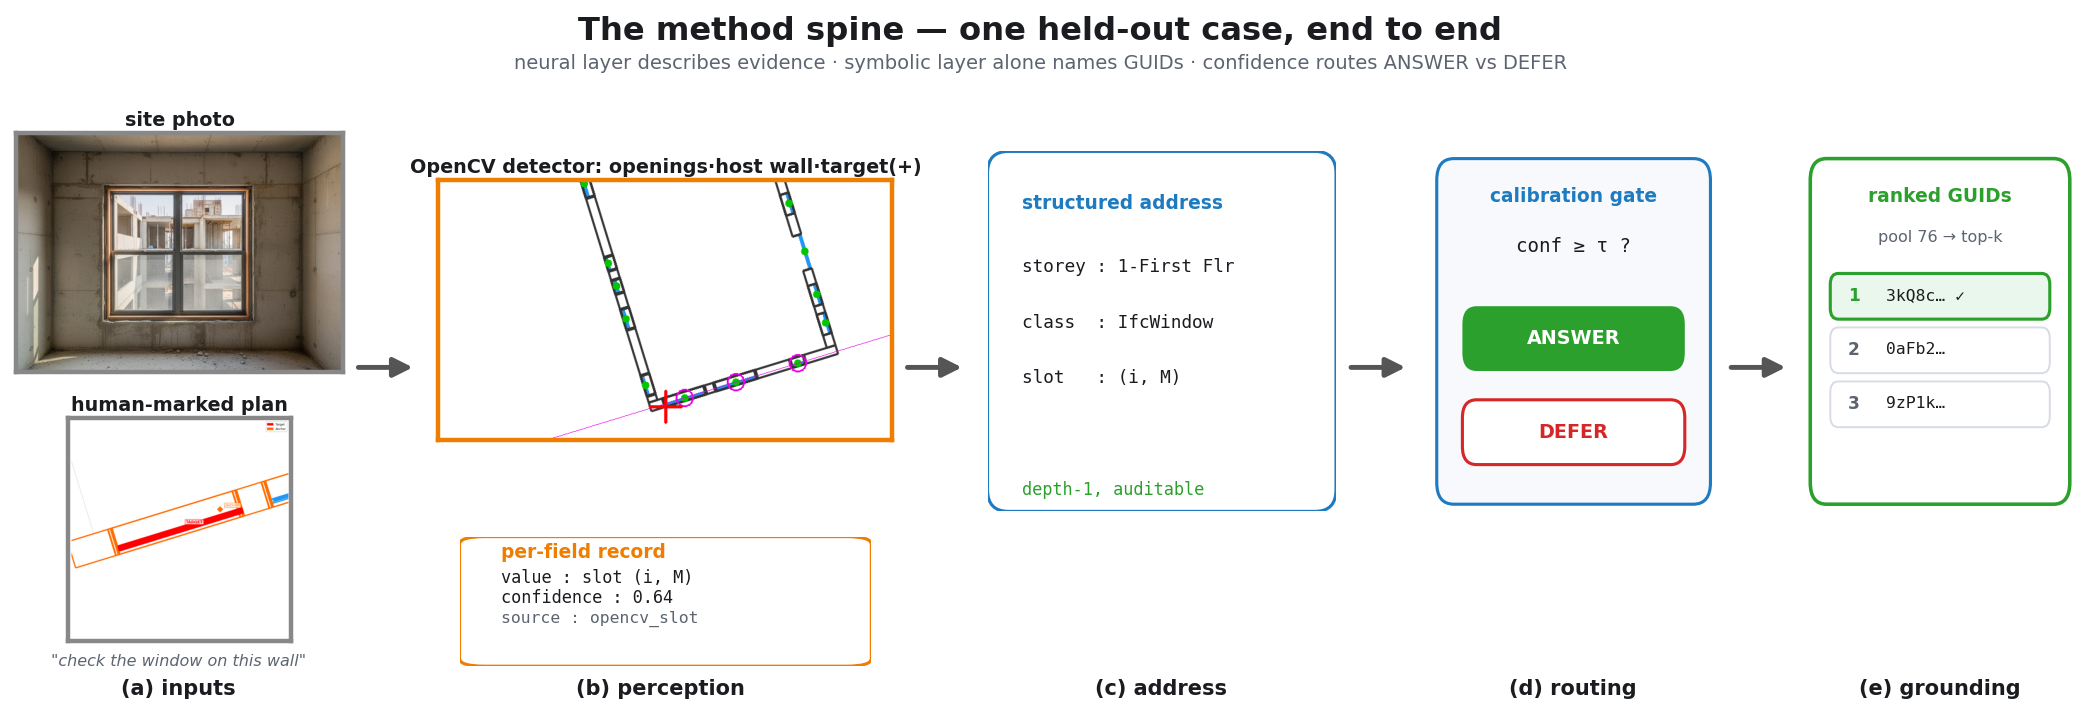
\includegraphics[width=\textwidth]{pipeline_shots.png}
  \caption{The method spine, on one held-out case (AP\_SK\_107), with the real artefacts as the
  centrepiece. \emph{(a)}~A site photograph, a human-marked plan (target wall in red, anchor in
  orange), and a short note enter. \emph{(b)}~The OpenCV slot detector's actual overlay reads the
  openings (green) along the host wall (magenta) and locates the target (red $+$), emitting a
  \texttt{\{value, confidence, source\}} record. \emph{(c)}~The depth-1 structured spatial-address
  record is assembled. \emph{(d)}~A calibration gate routes confident cases to \textsc{answer} and
  the rest to \textsc{defer}. \emph{(e)}~The address is matched against the IFC-graph pool to a
  ranked GUID shortlist. The neural layer describes evidence; the symbolic layer alone names GUIDs.}
  \label{fig:pipeline}
\end{figure}

\begin{figure}[ht]
  \centering
  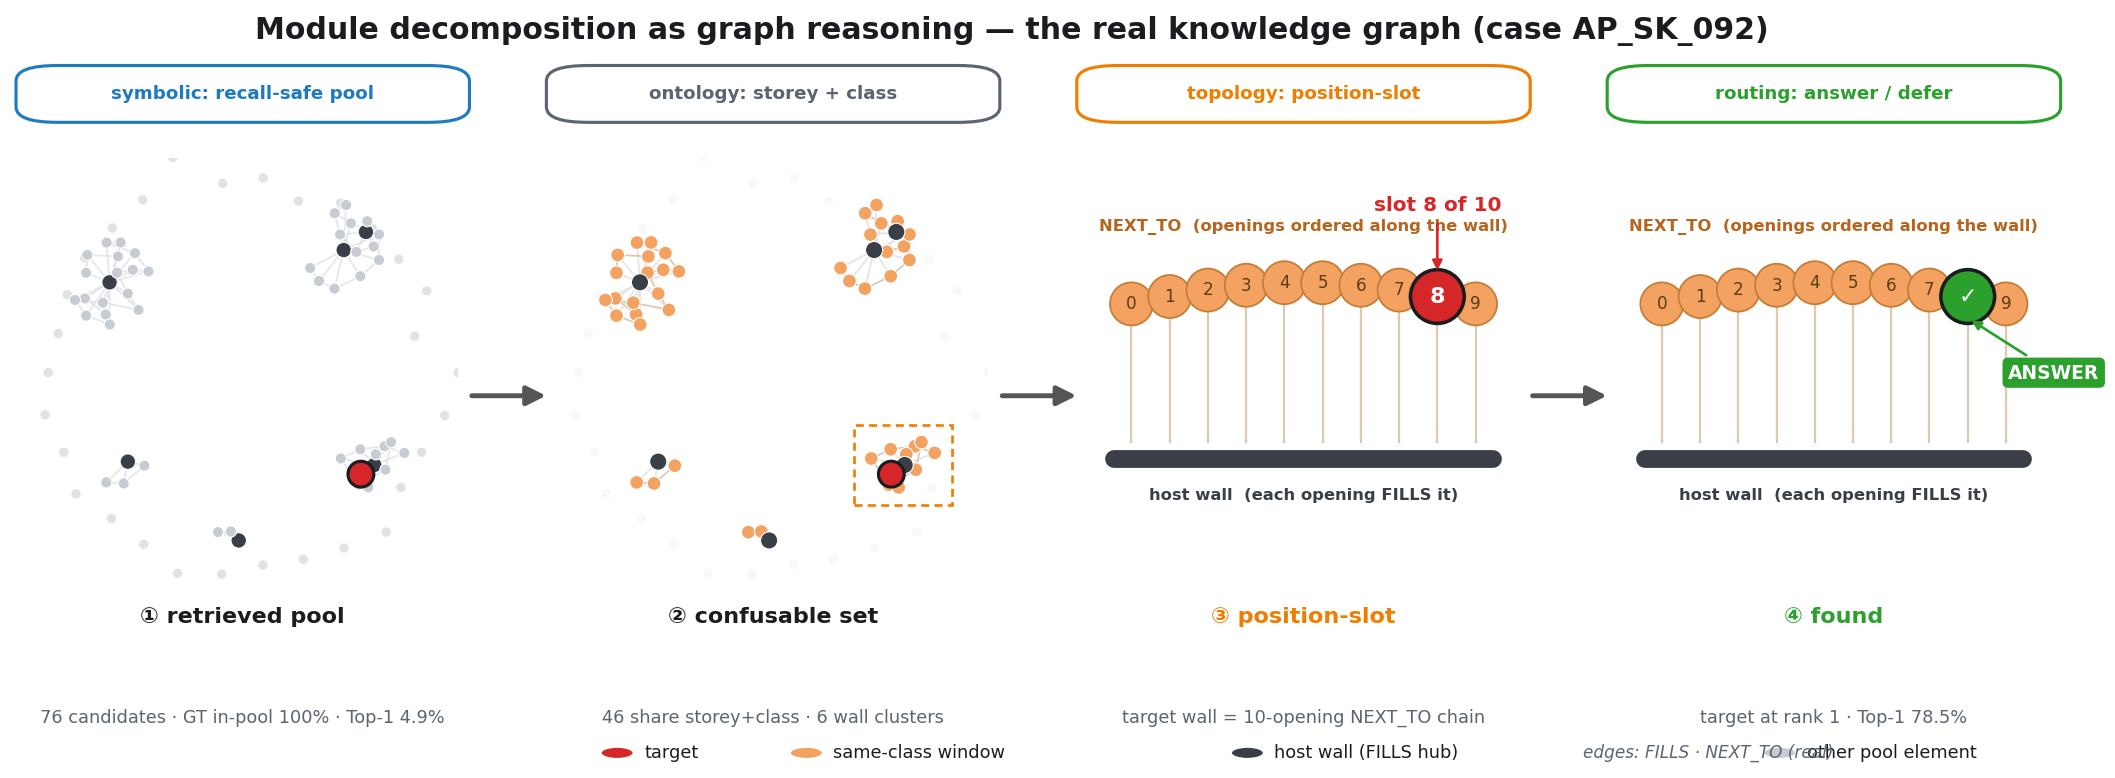
\includegraphics[width=\textwidth]{graph_reasoning.png}
  \caption{Module decomposition told as graph reasoning on one real held-out case (AP\_SK\_092, a
  window). The layout is the \emph{real} knowledge graph --- a force-directed layout on the actual
  \texttt{FILLS} (window$\to$host-wall hub) and \texttt{NEXT\_TO} (consecutive openings) edges, held
  fixed across all four panels so the same graph is progressively filtered. \textbf{(1)}~The symbolic
  layer returns a recall-safe pool of 76 candidates (ground truth in-pool 100\%) where Top-1 is only
  ${\sim}5\%$. \textbf{(2)}~46 of the 76 share the target's storey and IFC class, forming 6 host-wall
  clusters --- ontology cannot separate them, so ranking, not retrieval, is the problem.
  \textbf{(3)}~The target's host wall is a 10-opening \texttt{NEXT\_TO} chain; the position-slot (8 of
  10) re-weights the siblings (a soft prior --- no candidate removed). \textbf{(4)}~The target lands
  at rank 1 (oracle address Top-1 78.5\%). The target node (red) is tracked throughout.}
  \label{fig:decomp}
\end{figure}

\subsection{IFC parse engine: from a linear file to a query-ready graph}
\label{sec:ifc}

The symbolic substrate is built once per project by compiling the raw IFC file into a property graph
(IfcOpenShell $\to$ Neo4j), following the IFC-as-graph line \citep{zhu2023ifcgraph}. Beyond the
schema's containment hierarchy, the engine enriches the graph with the spatial topology the address
needs: \texttt{ON\_STOREY} from spatial containment, \texttt{FILLS} from
\texttt{IfcRelFillsElement}/\texttt{IfcRelVoidsElement} chains, \texttt{CONNECTS\_TO} from
\texttt{IfcRelConnectsPathElements} wall connectivity, and \texttt{ADJACENT\_TO} as generic proximity
(centroid distance under 1500\,mm) \citep{buildingsmart2024ifc4x3}. A graph database rather than a
vector store is a requirement, not a preference: the discriminating signal is multi-hop topology with
a deterministic schema, which embedding similarity cannot express. The reconstruction is validated
against the dataset's own skeleton --- the recovered wall \texttt{connection\_degree} matches ground
truth in 14 of 14 checked cases --- so the graph exists, correct and complete, on day one with no
human annotation: the cold-start property the system claims. Figure~\ref{fig:ifcengine} traces this
compilation: a flat STEP file whose only navigable structure is containment, the per-relation
enrichment rules with their edge counts on the studied project, and the resulting dense,
query-ready graph.

\begin{figure}[t]
  \centering
  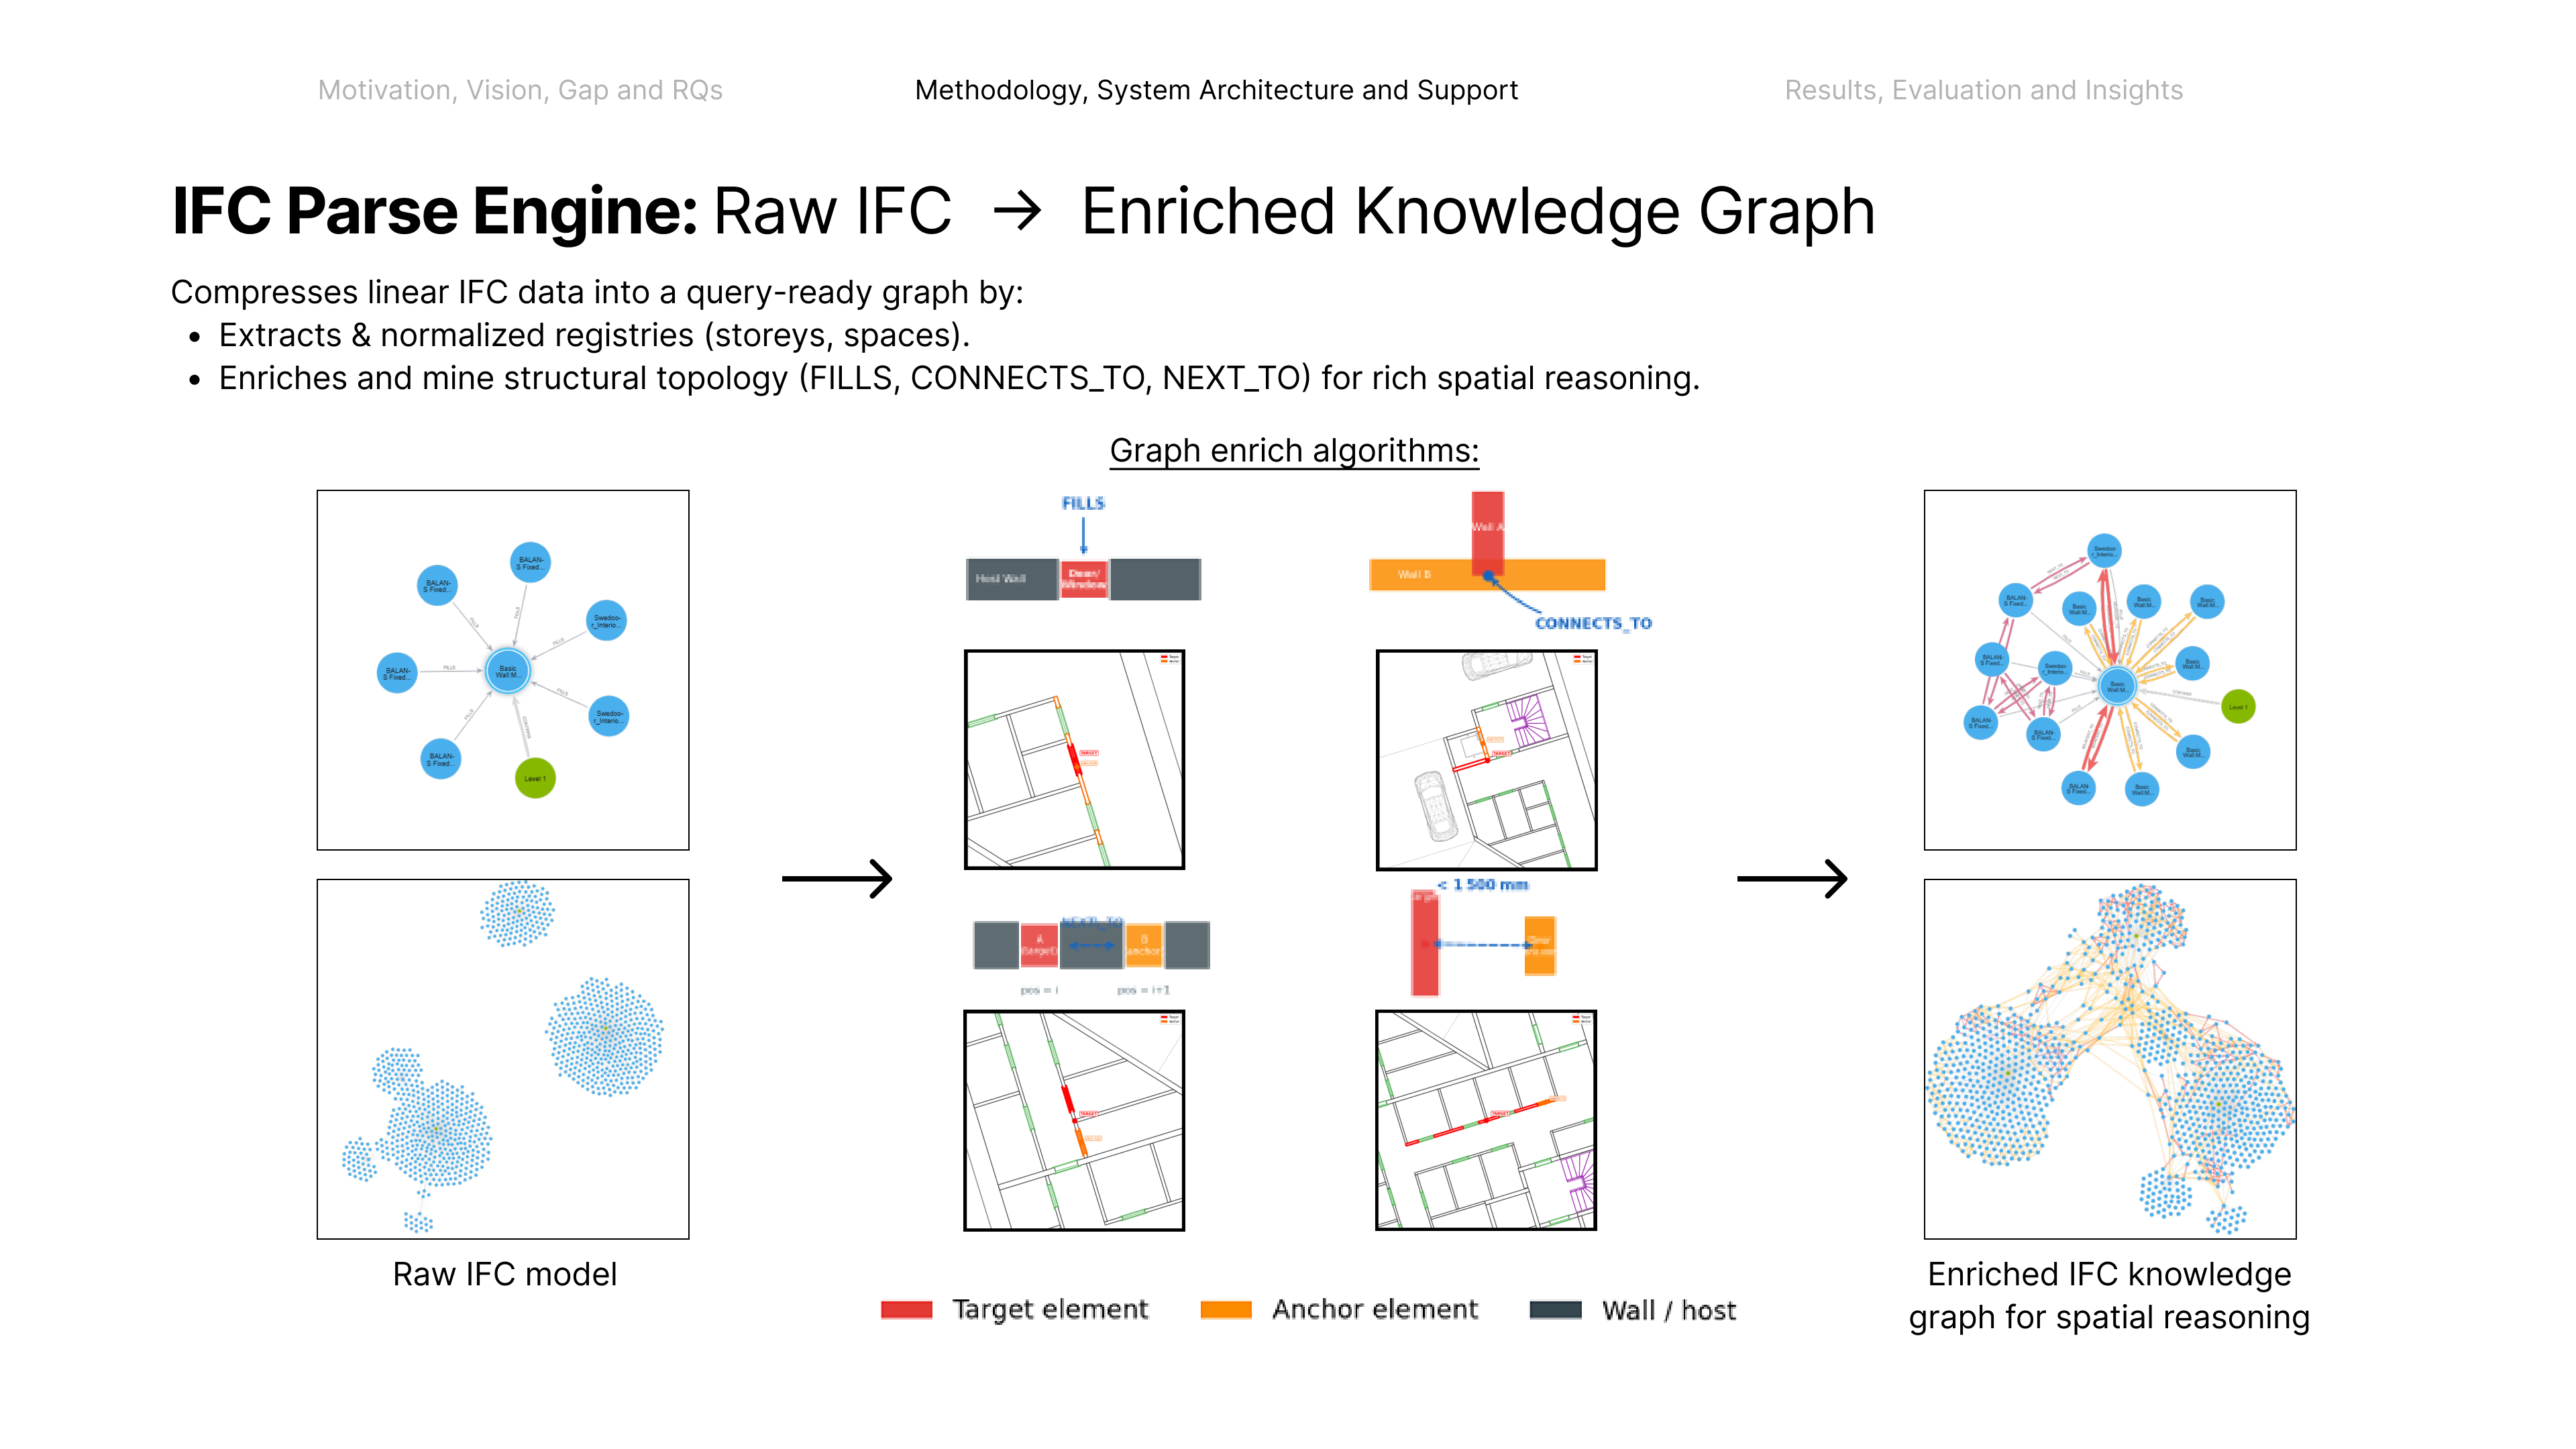
\includegraphics[width=\textwidth]{ifc_parse_slide.png}
  \caption{The IFC parse engine: from a raw IFC model (left) to an enriched, query-ready knowledge
  graph (right). The engine extracts and normalises the registries (storeys, spaces) and then mines
  structural topology --- \texttt{FILLS}, \texttt{CONNECTS\_TO}, \texttt{NEXT\_TO} --- shown by the
  per-relation enrichment insets (target element red, anchor orange, host/wall dark). The local
  containment-only graph cannot separate identical siblings; the enriched graph carries the relational
  structure the spatial address queries.}
  \label{fig:ifcengine}
\end{figure}

\subsection{Neural layer: a fine-tuned VLM as the perception engine}
\label{sec:vlm}

The perception engine is Qwen2.5-VL-7B with LoRA adapters (rank 32 in the strongest configurations,
targeting Q/K/V/O and MLP layers across both the vision encoder and the language model), chosen for
stable JSON emission and native dynamic resolution. It reads the photo, the note, and the plan crop
and emits a structured contract --- \texttt{\{storey\_name, ifc\_class,
spatial\_relations:[\{predicate, object\_type, direction\}]\}} --- and nothing else: \emph{it
describes, it never queries} (Figure~\ref{fig:vlmimpl}). Fine-tuning on the synthetic corpus is what
makes the spatial fields exist at all: spatial-direction accuracy reaches 82\% where zero-shot
prompting scores ${\sim}0\%$ (this 82\% and the G-series ablation below are prior thesis measurements,
not re-run on this repo's harness), and the coarse fields (storey, \texttt{ifc\_class}) saturate at
100\% versus 30--63\% zero-shot. The G-series ablation also exposes a
multi-task capacity trade-off under a fixed adapter rank: under-resourced adapters collapse on spatial
extraction while the coarse fields stay saturated, so topology-specific supervision and added
position-context capacity are needed to recover spatial fingerprints --- and, as the per-field profile
in \secref{sec:eval-neural} shows, the finest discriminating fields do not survive fine-tuning at all,
which is why they are delegated to the specialists below.

\begin{figure}[ht]
  \centering
  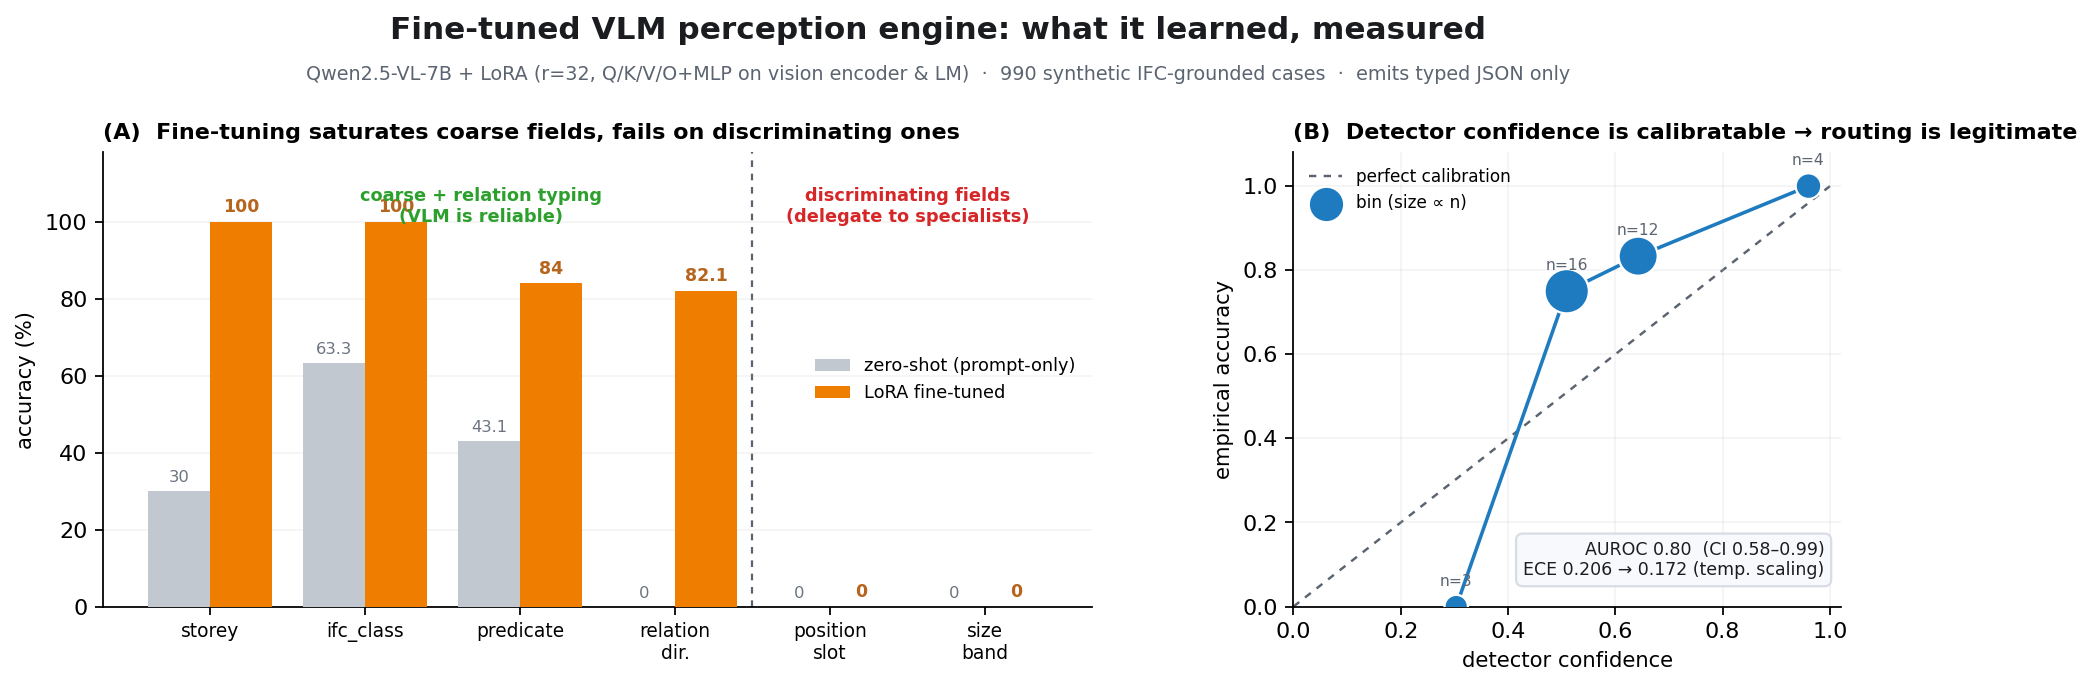
\includegraphics[width=\textwidth]{vlm_finetune.png}
  \caption{The fine-tuned VLM perception engine, measured. \emph{(A)}~Per-field accuracy, ordered
  coarse$\to$discriminating, zero-shot prompt-only versus LoRA fine-tuned: fine-tuning saturates the
  coarse prefix (storey, \texttt{ifc\_class} from 30/63\% to 100\%) and learns relation typing
  (direction ${\sim}0\%\to82\%$), but the \emph{discriminating} address fields (position-slot, size
  band) stay at 0\% even fine-tuned --- the evidence that motivates delegating them to deterministic
  specialists. \emph{(B)}~The realized detector's confidence is calibratable (reliability diagram;
  AUROC 0.80, ECE $0.206\!\to\!0.172$ after temperature scaling), which is what makes
  confidence-routing legitimate. (No training-step loss curve is shown: per-field gain, held-out
  generalisation, and calibration are the meaningful evidence that a structured-extraction adapter has
  learned.)}
  \label{fig:vlmimpl}
\end{figure}

\subsection{Synthetic data pipeline: supervision with zero real labels}
\label{sec:synth}

Cold-start means no real paired data, so supervision is manufactured from the model itself in three
stages. \emph{Stage 1 --- IFC structure mining:} IfcOpenShell traversal plus spatial-relationship
computation yields, for every element, its ground-truth address and relational context. \emph{Stage 2
--- visual synthesis:} Blender renders scenes with deliberate hard negatives --- identical-looking
adjacent rooms --- so the model cannot shortcut on appearance. \emph{Stage 3 --- text generation:} an
LLM writes site-note queries at varying specificity, and an LLM-as-judge filter removes degenerate
cases. The output is 990 training cases on the studied project and a 60-case held-out benchmark (the
evaluation set throughout \secref{sec:eval}).

\subsection{Symbolic layer: deterministic query compilation with a recall-safe cascade}
\label{sec:symbolic}

The constraint contract compiles into Cypher through nine predefined query strategies (spatial
triplet, continuous span, space+type, \ldots); the VLM never generates Cypher
(\secref{sec:rationale}). Execution follows a cascade that is recall-safe by construction: strict
constraints first, then loosen one constraint at a time, with a storey+type safety net guaranteeing a
non-empty pool. The pool is then \emph{never} hard-filtered further --- the measured reason is in
\secref{sec:eval-union} --- and ranking inside the pool is delegated to the spatial address.

\subsection{The spatial address, deterministic specialists, and calibrated routing}
\label{sec:address}

The element that closes the loop is the \textbf{type-conditional spatial address}: the minimal
descriptor set that identifies an element within its confusable set $C(e)$ --- the pool elements
sharing its storey and IFC class --- subject to two deployment constraints: it must be
\textbf{IFC-computable} (derivable from the model with no labels) and \textbf{image-recoverable}
(estimable from photo and plan). The address is class-conditional. \emph{Fillers} (windows, doors) are
identified by the \textbf{position-slot} $(i, M)$: the $i$-th of $M$ openings ordered along the host
wall, numbered in an image-coordinate convention (a representational prerequisite quantified in
\secref{sec:eval-realized}). \emph{Walls} are identified by a \textbf{connectivity fingerprint}
(\texttt{connection\_degree}, \texttt{hosted\_opening\_count}, \texttt{length\_band},
\texttt{is\_external}). Relational context is \emph{compiled into the node} at ingestion --- the
depth-1 sub-graph and the distilled node attributes carry the same information --- so the runtime
extractor recovers at most one hop (the depth law, \secref{sec:eval-depth}).

Recovery of the discriminating fields is delegated to \textbf{deterministic visual specialists}: an
OpenCV detector that color-segments the plan's openings and orders them along the host wall to read
the position-slot, and a ResNet size head for dimension bands --- both of which outperform the trained
VLM on exactly these sub-tasks. Every extracted field, from every source, is emitted as a uniform
record \texttt{\{value, confidence, source\}} --- the contract invariant. A routing policy consumes the
contract: the recovered slot enters the rerank as a confidence-weighted prior inside the recall-fixed
pool, and a low-confidence extraction routes to \textbf{defer} (``here are the candidates'') rather
than to a confident wrong answer. The premise that confidence may route at all is gated on calibration
\citep{guo2017calibration} and measured, not assumed (\secref{sec:eval-realized}).

\section{Evaluation \& Results}
\label{sec:eval}

\subsection{Setup, metrics, and staging}
\label{sec:eval-setup}

All numbers are measured on the held-out benchmark of the studied project (Tier-3; $n=60$ cases / 59
elements, of which 35 are addressable fillers). The split is region-disjoint by construction, but a
data audit found \textbf{element-level leakage}: 12 of the 59 held-out target elements (9 fillers, 3
walls) also appear as training targets under a different render, because an element can sit in two
regions. We disclose this directly and note that it cannot affect the headline results by
construction: the oracle diagnostics (\secref{sec:eval-oracle}, \secref{sec:eval-depth}) read only
the IFC graph and learn nothing, and the realized position-slot result (\secref{sec:eval-realized})
uses a \emph{deterministic} OpenCV detector with no trained weights --- both are leakage-proof. The
only learned component touched by the split is the per-field VLM profile
(\secref{sec:eval-neural}); re-profiling on the leakage-clean 48-case subset leaves it unchanged
(storey/class $100\%$, position-slot/size $0\%$), so the architectural conclusion does not depend on
the leaked cases. We structure the
evaluation in stages: first, an \emph{oracle} experiment establishing the symbolic-layer ceiling under
perfect extraction (\secref{sec:eval-oracle}); second, neural extraction accuracy per field
(\secref{sec:eval-neural}); third, how noisy signals combine without destroying recall
(\secref{sec:eval-union}); fourth, the realized extractor with calibrated, selectively-predictive
routing (\secref{sec:eval-realized}); fifth, the depth analysis (\secref{sec:eval-depth}); and last,
failure decomposition and workflow-facing cost (\secref{sec:eval-failure}). This staging separates
symbolic retrieval quality from neural extraction quality --- the two failure modes require different
fixes, and conflating them produces misleading aggregate metrics. We report \textbf{GT-in-Pool} as the
primary retrieval metric rather than Top-1, because Top-1 conflates retrieval failure (element never
in the pool) with ranking failure (element in the pool but ranked poorly); guaranteed retrievability is
the architectural contribution, and ranking is where the spatial address acts. Table~\ref{tab:main} consolidates the headline numbers; the remainder of
this section derives and explains each block.

\begin{table}[ht]
  \centering
  \small
  \begin{tabular}{lrrrr}
    \toprule
    Method & GT-in-Pool & Top-1 & Top-10 & MRR@10 \\
    \midrule
    \multicolumn{5}{l}{\emph{External baselines, full held-out pool ($n=60$)}} \\
    \quad Lexical (BM25)                          & 100 & 1.7  & 15.6 & 0.058 \\
    \quad Dense (MiniLM)                          & 100 & 1.7  & 25.0 & 0.108 \\
    \quad Zero-shot VLM --- full pool             & 100 & 3.3  & 15.0 & 0.086 \\
    \quad Zero-shot VLM --- sibling shortlist     & 100 & 3.3  & 20.0 & 0.097 \\
    \midrule
    \multicolumn{5}{l}{\emph{Our pipeline, realized end-to-end ($n=60$)}} \\
    \quad G8 extraction $\to$ deterministic retrieval & ${\sim}100$ & 6.7 & 30.0 & 0.110 \\
    \midrule
    \multicolumn{5}{l}{\emph{Oracle ceiling, same pools ($n=60$)}} \\
    \quad Coarse: storey $+$ class                & 100 & 4.9  & 31.5 & 0.137 \\
    \quad \quad $+$ \texttt{object\_type}         & 100 & ---  & 76.0 & ---   \\
    \quad \quad $+$ structured spatial address    & 100 & \textbf{78.5} & \textbf{98.1} & \textbf{0.854} \\
    \midrule
    \multicolumn{5}{l}{\emph{Realized address, addressable fillers ($n=35$)}} \\
    \quad Modal-prior slot (floor)                & 100 & 6.6  & ---  & ---   \\
    \quad OpenCV slot $+$ soft rerank             & 100 & \textbf{67.6}$_{[53.6,81.6]}$ & 80.9 & --- \\
    \bottomrule
  \end{tabular}
  \caption{Consolidated held-out results. Every method ranks the \emph{same} retrieved pools with the
  ground truth in-pool throughout (GT-in-Pool, \%), so the table isolates \emph{ranking}, not
  retrieval. Top-1/Top-10/MRR in \%. External text retrieval and a zero-shot Qwen2.5-VL-7B reranker
  (base model, no adapter) stay at single-digit Top-1 --- the VLM at chance --- while the oracle
  structured address reorders the identical pool to 78.5\%. The realized filler block shows how much
  survives a real detector: one deterministic specialist lifts Top-1 from the 6.6\% floor to 67.6\%
  (bootstrap 95\% CI in subscript); deferring the least-confident ${\sim}20\%$ further lifts the
  answered subset to 80.6\% (\secref{sec:eval-realized}). Dashes mark quantities not measured for that
  row.}
  \label{tab:main}
\end{table}

\subsection{Oracle experiment: the symbolic ceiling, and where discrimination lives}
\label{sec:eval-oracle}

Under perfect extraction the symbolic layer retains the target in \textbf{100\% of cases}
(GT-in-Pool) and compresses the live pool along the fingerprint ladder --- from $1{,}233$
elements (whole-model) to 46 (storey+class) toward single digits as spatial constraints are added. The architecture is therefore provably sound; the question is where,
inside the pool, the discriminating information lives.

\paragraph{The coarse floor saturates.} Restricting to the target's storey and IFC class leaves a
median confusable set of 46 (mean 112) and an oracle Top-1 of only \textbf{4.9\%} --- \emph{below} the
realized end-to-end reranker (6.7\%) and equal to it on Top-10 (31.5\% vs.\ 30.0\%). Ontology is
necessary but cannot separate same-class siblings: it is the floor, not the discriminator. Adding the
richest attribute (the family/type string \texttt{object\_type}) shrinks the confusable set to a
median of 13 ($3.8\times$) and lifts oracle Top-10 to 76\%, but uniquely identifies only 2 of 60
targets. What remains is the irreducibly \emph{relational} residue.

\paragraph{The type-conditional address closes it.} Supplied at an oracle level, the class-conditional
address of \secref{sec:address} takes the real retrieved pool from a coarse Top-1 of 4.9\% to
\textbf{78.5\%}, and Top-10 from 31.5\% to \textbf{98.1\%} (MRR $0.137 \to 0.854$), at zero recall
cost. The gain decomposes exactly along the type-conditional split --- fillers reach Top-1
\textbf{91.0\%} (position-slot), walls \textbf{64.2\%} (connectivity fingerprint; within same-storey
walls the fingerprint collapses a median confusable set of $110 \to 2$, uniquely identifying 10 of 22
walls where \texttt{object\_type} identifies none). No uniform descriptor achieves this: the
position-slot is meaningless for a wall, the fingerprint degenerate for a window. Generic retrieval
baselines confirm the gap is not an artifact of our own pipeline. Lexical and dense retrievers plateau
at Top-1 1.7\% (Top-10 15.6\% / 25.0\%) on the same pools, and a \emph{zero-shot} Qwen2.5-VL-7B
reranker --- the same backbone our extractor fine-tunes, given the marked site photo, the marked
floorplan, and the candidate pool --- stays at chance: Top-1 3.3\% over the full pool and 2.9\% on
fillers even when the pool is pre-filtered to the same-storey, same-class confusable set
(per-case chance 1.8--2.4\%; candidates are shuffled so that copying the list order scores at chance,
which is what the model does). On those same pools the oracle spatial address reaches 78.5\%
(Figure~\ref{fig:external}). A strong general VLM cannot recover the relational slot from the image
alone; the structured address, not the backbone, is what discriminates identical siblings.

\begin{figure}[ht]
  \centering
  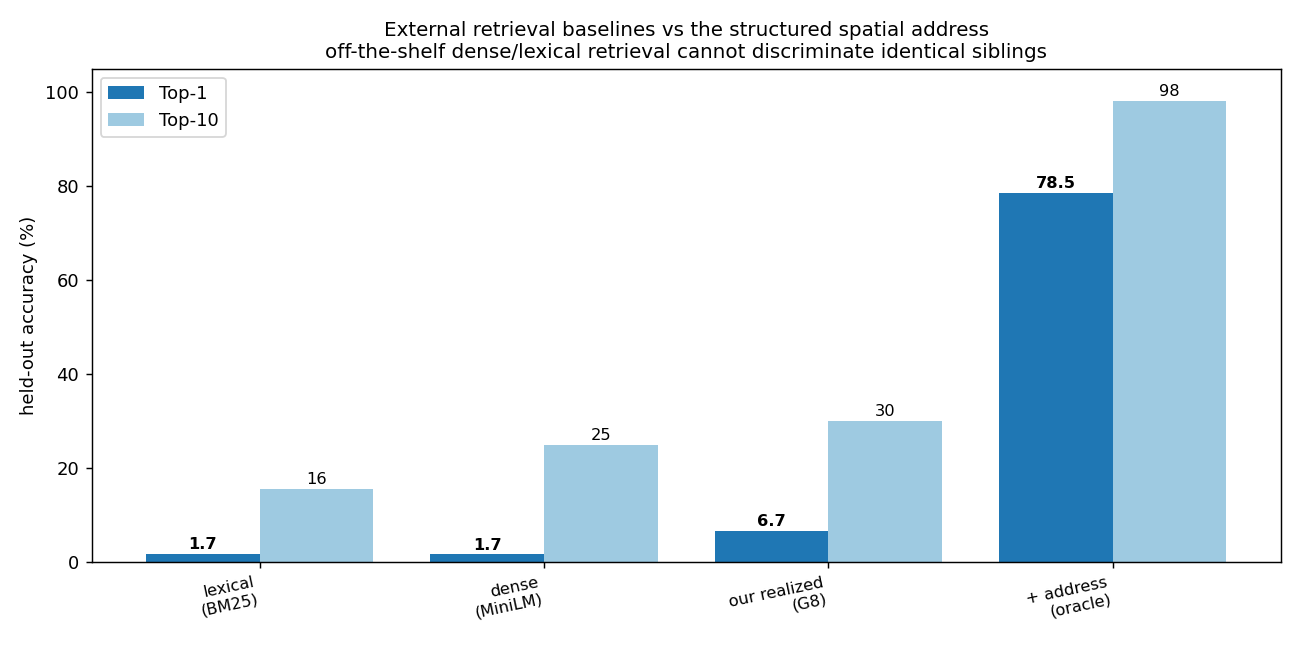
\includegraphics[width=0.85\textwidth]{external_baseline.png}
  \caption{Baselines against the oracle ceiling on identical pools. Lexical and dense text retrieval,
  a zero-shot Qwen2.5-VL-7B reranker (base model, no adapter; both the full pool and the
  same-storey/class sibling shortlist), and the deployed G8 pipeline all plateau in single-digit
  Top-1 --- the zero-shot VLM at chance --- with the ground truth in-pool throughout; the oracle
  spatial address reorders the same pool to 78.5\%/98.1\%. The bottleneck is ranking inside the pool,
  and the missing signal is the relational address.}
  \label{fig:external}
\end{figure}

\subsection{Neural extraction quality: what the fine-tuned VLM does and does not recover}
\label{sec:eval-neural}

Per-field evaluation shows fine-tuning works where it was aimed: against zero-shot prompting
(\texttt{ifc\_class} 63.3\%, storey 30.0\%), the fine-tuned models saturate both at \textbf{100\%},
reach predicate slot-accuracy 82.8--86.2\% versus 43.1\%, and lift relation direction to 82.1\% versus
${\sim}0\%$. End-to-end, however, the best configuration delivers
Top-10 30.0\% / Top-1 6.7\% / MRR@10 0.110 --- with the target in the pool ${\sim}100\%$ of the time.
The decisive diagnostic is the held-out per-field re-profile (Figure~\ref{fig:vlm}): the VLM is
saturated on the \emph{coarse prefix} (storey, class --- exactly the fields the oracle shows are
non-discriminating) and recovers the \emph{discriminating} structured fields at \textbf{0\%} (the
position-slot and the size band), and emits a relation-direction field in 57\% of held-out cases
(this 57\% is an \emph{emission rate} --- whether any direction is produced --- not the 82\%
direction \emph{accuracy} reported above on the thesis evaluation set; the two numbers measure
different quantities and are not comparable). The conclusion is
architectural, not ``fine-tune harder'': delegate the slot and size to deterministic visual
specialists, keep the VLM on the coarse prefix and relation typing where it is reliable. This is the
neuro-symbolic interface in practice --- learn where the network is reliable, compute
deterministically where it is not \citep{mao2019nscl}.

\begin{figure}[ht]
  \centering
  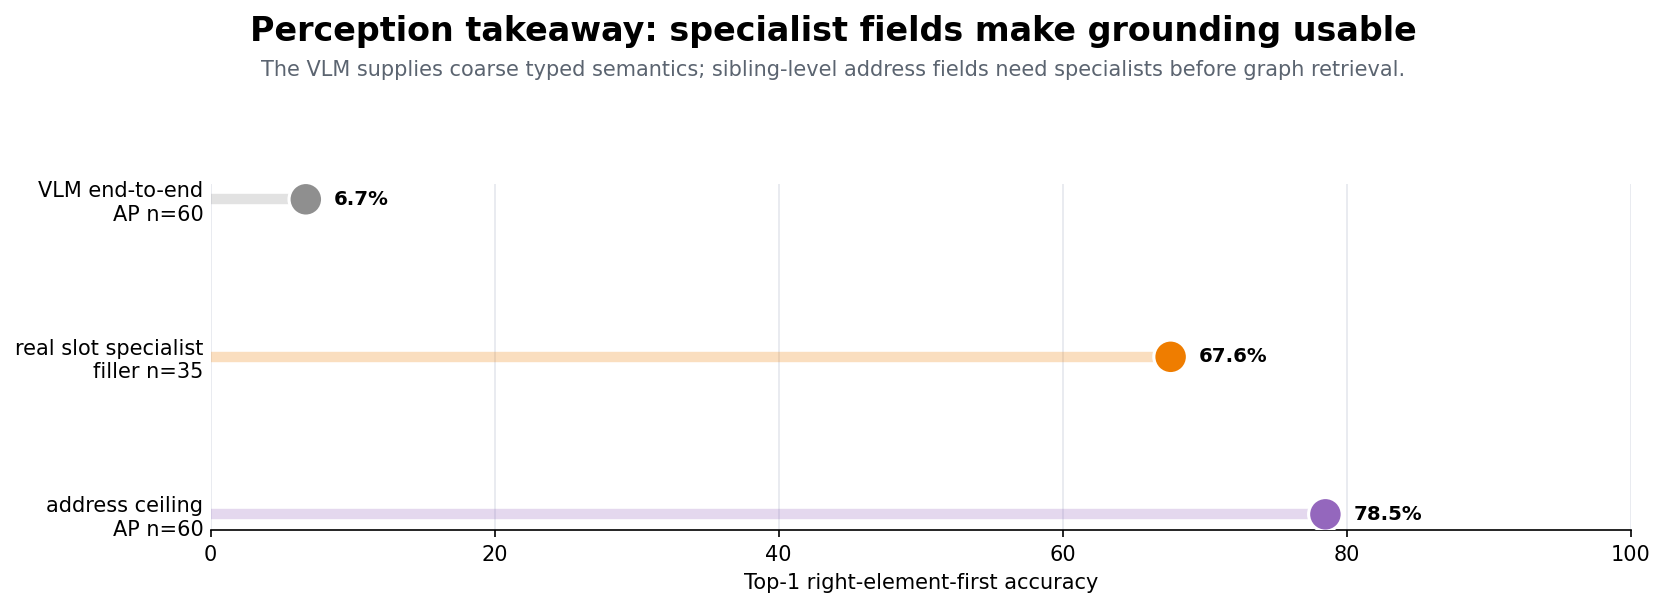
\includegraphics[width=0.85\textwidth]{vlm_profile.png}
  \caption{Perception takeaway: per-field re-profile of the fine-tuned VLM on the held-out set. The
  coarse prefix (storey, class) saturates; the discriminating fields (position-slot, size) are
  recovered at 0\% --- motivating delegation to deterministic specialists.}
  \label{fig:vlm}
\end{figure}

\subsection{Combining signals: union, never intersection}
\label{sec:eval-union}

How should a mature signal (storey+type) combine with an immature one (spatial topology)? The strategy
ablation is unambiguous: the \textbf{union} of constraint sets is the only strategy that preserves
full GT-in-Pool while still gaining the spatial constraints' compression and ranking benefit; hard
intersection over-prunes under noisy extraction, and spatial-only is too brittle. The measurement says why: treating each extracted field as a hard
filter multiplies per-field recalls --- with measured single-field reliabilities (storey
$\approx 0.66$, class $\approx 0.50$), a hard conjunction over the attribute fields collapses joint
recall toward $\prod r \approx 0.009$. The filter evicts the ground truth far more often than it
removes a distractor. The resolution is to relocate determinism: \textbf{the executor is deterministic
given the structured record; the ranking is a calibrated soft prior inside a recall-fixed pool.} The
address never removes a candidate; it re-weights one. Recall stays at 100\% by construction, and the
unreliable signal is spent only on ordering. As a design principle this generalizes: when combining
mature and immature signals, union --- intersection amplifies extraction error and destroys recall.

\subsection{Realizing the address: one specialist, calibrated, selectively predictive}
\label{sec:eval-realized}

The oracle ceiling is a statement about information; this section measures how much survives a real,
imperfect detector. The honest floor is stark: the fine-tuned reranker emits position as free text and
recovers a usable slot in \textbf{0 of 35} held-out fillers; even a modal-prior slot guess reaches
only 6.6\%. We report four results.

\paragraph{(1) One realizable extractor closes most of the gap.} The OpenCV position-slot detector
recovers the opening count exactly in 83\% of cases (29/35) and the full slot in 74\% (joint
$(i,M)$). Fed into the soft rerank, it lifts filler Top-1 from the 6.6\% floor to \textbf{67.6\%}
(bootstrap 95\% CI $[53.6, 81.6]$, $n=35$) and Top-10 to 80.9\%, at zero recall cost. The residual
error concentrates in the ordering index, not in the perception of the openings. The wide interval is
a direct consequence of the small addressable set and is reported, not smoothed over. The detector's
three pixel thresholds are not a knife-edge fit: sweeping each $\pm25\%$ leaves realized Top-1 in
$[55.1, 83.1]$ (never near the 6.6\% floor), two of the three are inert, and only the same-wall
perpendicular band matters --- and the deployed value is mid-range, not tuned to the peak.

\paragraph{(2) A representational prerequisite: the address must be image-recoverable.} The
ground-truth slot in the source data is numbered along each wall's IFC local-X axis --- a modelling
artefact invisible in any image. Scored against that convention, detector and ground truth disagree on
16 of 35 fillers, \emph{all} exact mirrors $i \mapsto M{-}1{-}i$; under an image-coordinate convention
the disagreement vanishes and joint accuracy rises from an apparent 34\% to the true 74\%. An address
field is realizable only if it is defined in a frame the evidence carries --- a substantive design
constraint, not bookkeeping. The same constraint explains a negative result: the wall fingerprint's
load-bearing fields depend on IFC wall-\emph{instance} boundaries that collinear instances erase in
the floorplan poch\'e (length-band recovery 5/17, realized Top-1 $\approx$ floor), so the wall address
is oracle-discriminative but \emph{not} image-realizable, and realization is scoped to the filler
slot.

\paragraph{(3) The confidence is calibratable --- and reweighting is a measured no-op.} Routing is
only legitimate if confidence tracks correctness \citep{guo2017calibration}. On the held-out fillers
the raw detector confidence is positively discriminative (AUROC \textbf{0.80}, bootstrap 95\% CI
$[0.58, 0.99]$) and moderately mis-calibrated (ECE 0.206, 95\% CI $[0.09, 0.32]$); temperature
scaling reduces it to 0.172 (Figure~\ref{fig:caldiag}). The intervals are wide --- at $n=35$ the
calibration evidence is suggestive, not conclusive, and we treat the gate as a measured operating
point rather than a precise estimate. But
the calibrated weight does \emph{not} pay off as a rerank weight: because the slot is the finest
tiebreaker inside a storey$\times$class bucket, any strictly-positive weight induces the identical
ordering --- hard match, raw weight, and calibrated weight all yield the same 67.6\%. We report this
no-op rather than bury it.

\paragraph{(4) The payoff is selective prediction.} The calibrated confidence pays off as a deferral
threshold: sweeping it traces a coverage--accuracy curve (Figure~\ref{fig:rerank}), and deferring the
least-confident ${\sim}20\%$ of cases lifts Top-1 on the answered subset from 67.6\% to
\textbf{80.6\%} \citep{geifman2017selective}. A worked case (Figure~\ref{fig:demo}) shows the
mechanism: the detector predicts slot 1 of 10 where the truth is 8 of 10 --- an error --- but its
calibrated confidence (0.05) is below threshold, so the case routes to \emph{defer} and surfaces the
candidates instead of a confident wrong GUID. For a triage tool with downstream consequence, this is
the correct behavior, and the coverage--accuracy curve, not a point estimate, is the honest report.

\begin{figure}[ht]
  \centering
  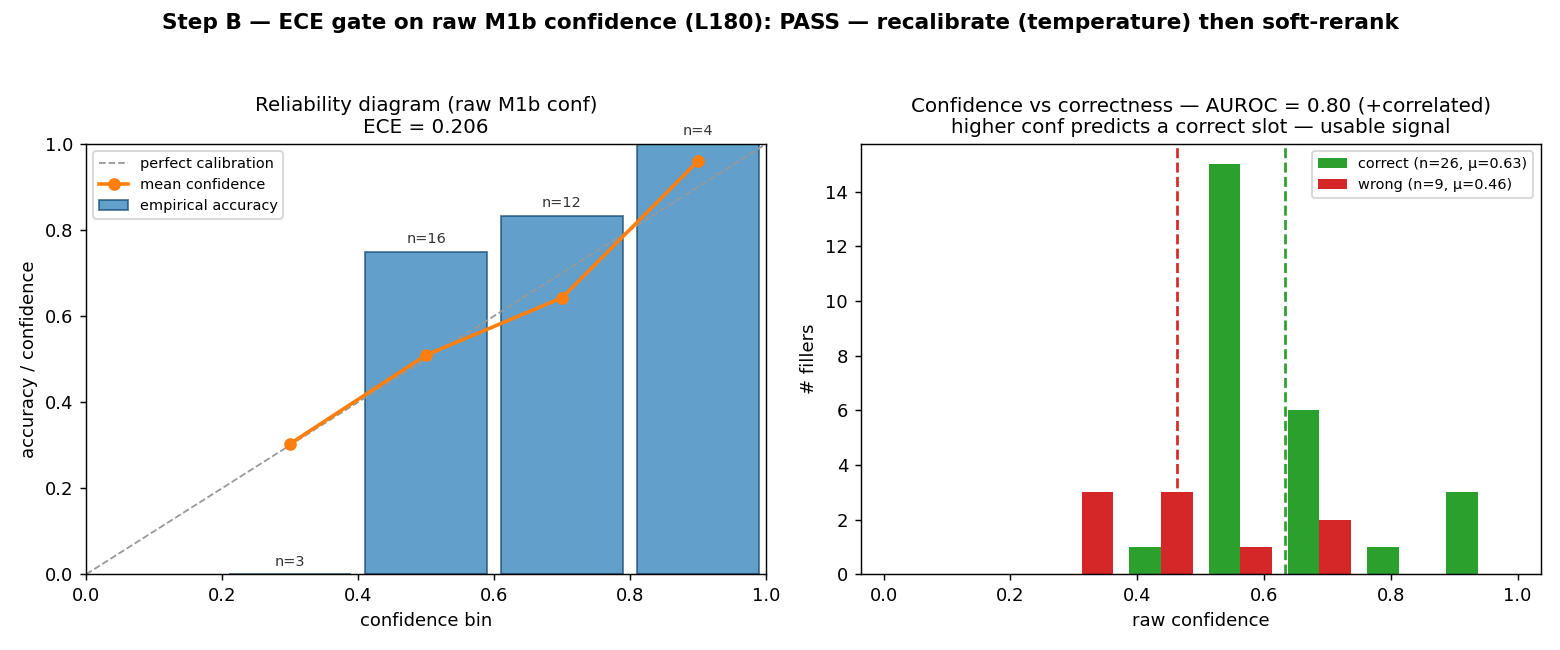
\includegraphics[width=0.85\textwidth]{calibration_diag.png}
  \caption{Calibration gate. Raw detector confidence is positively discriminative (AUROC 0.80) and
  moderately mis-calibrated (ECE 0.206); temperature scaling reduces ECE to 0.172.}
  \label{fig:caldiag}
\end{figure}

\begin{figure}[ht]
  \centering
  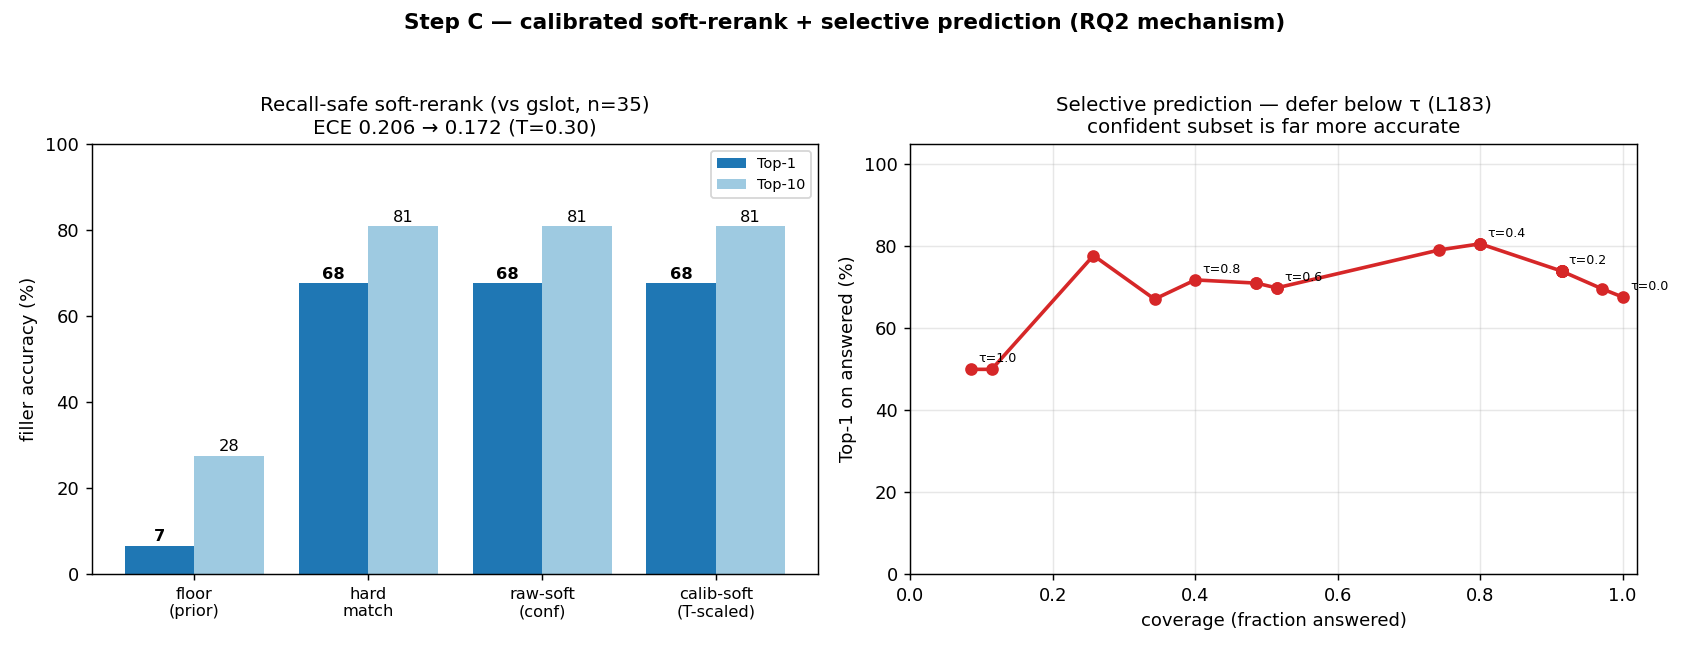
\includegraphics[width=0.85\textwidth]{calibrate_rerank.png}
  \caption{Selective prediction. Sweeping the deferral threshold traces a coverage--accuracy curve;
  deferring the least-confident ${\sim}20\%$ lifts answered-set Top-1 from 67.6\% to 80.6\%.}
  \label{fig:rerank}
\end{figure}

\begin{figure}[ht]
  \centering
  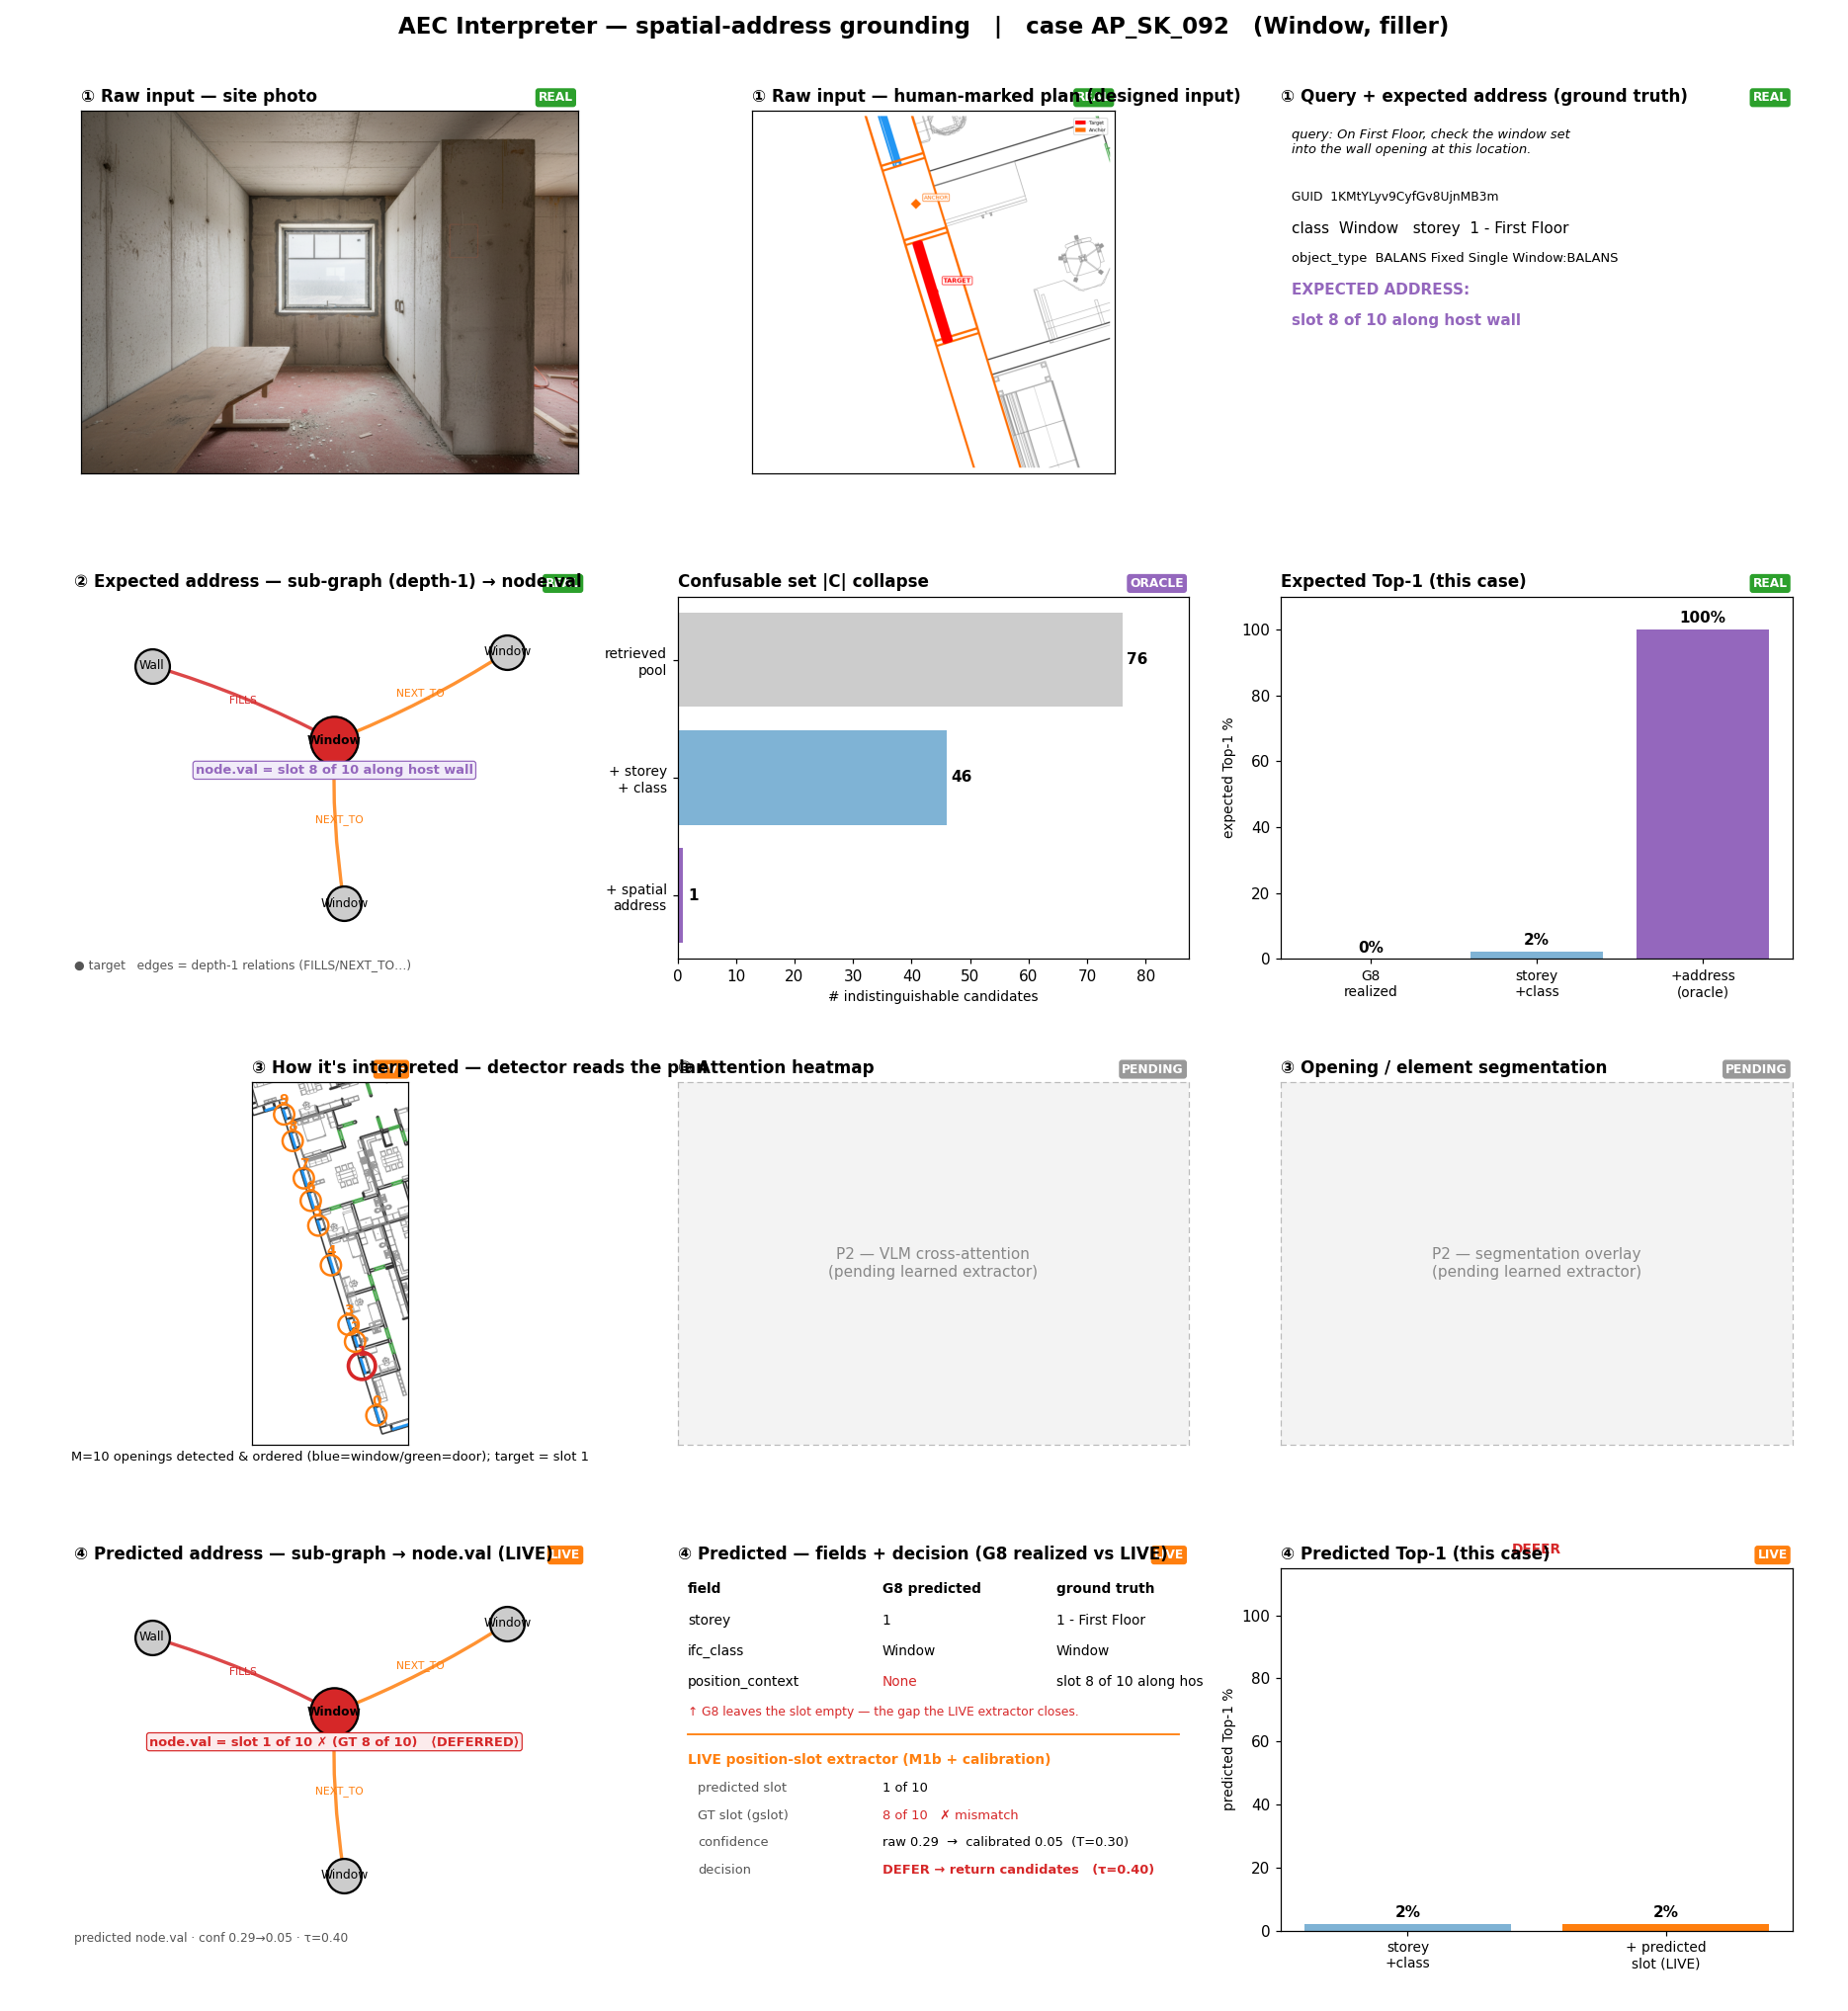
\includegraphics[width=\textwidth]{case_AP_SK_092.png}
  \caption{A worked DEFER case. The detector predicts slot 1 of 10 where the truth is 8 of 10, but
  its calibrated confidence (0.05) is below threshold: the case routes to defer and surfaces the
  candidate pool rather than emitting a confident wrong GUID.}
  \label{fig:demo}
\end{figure}

\subsection{The depth law: relational context saturates at one hop}
\label{sec:eval-depth}

Where should relational context live --- extracted deep at inference, or compiled into the node? Under
an oracle, deeper context keeps shrinking the confusable set (a Weisfeiler--Leman-style refinement
toward singletons). But the relations must be recovered from an image, and per-hop extraction
reliability falls as $0.40 \to 0.05 \to 0$, so the \emph{realizable} confusable set saturates
immediately (Table~\ref{tab:depth}, Figure~\ref{fig:depth}): median 13 (attributes) $\to$
\textbf{8.2} at one hop $\to$ 8.1 at two and three. This is the depth law --- deeper context is
informative but not recoverable --- and its failure mode is the documented error compounding of
multi-hop reasoning over knowledge graphs \citep{chakraborty2024multihop}. The training side
corroborates it: supervising depth-3 chains yielded ${\approx}0$ realizable improvement and \emph{cost}
capacity --- under a fixed LoRA rank, depth-$\ge 2$ chains degraded the coarse \texttt{ifc\_class}
recovery, and the deep-chain extraction itself ran at ${\sim}5\%$ and hurt end-to-end performance by
${\sim}13$ points. The prescription is subtractive: stop training deep
chains, compile depth into the node, extract at depth $\le 1$.

\begin{table}[ht]
  \centering
  \begin{tabular}{lc}
    \toprule
    relational depth & realizable median $|C|$ \\
    \midrule
    attributes only (depth 0) & 13 \\
    \textbf{+ 1 hop} & \textbf{8.2} \\
    + 2 hops & 8.1 \\
    + 3 hops & 8.1 \\
    \bottomrule
  \end{tabular}
  \caption{Realizable median confusable-set size by relational depth (held-out set). All realizable
  discrimination is captured at one hop.}
  \label{tab:depth}
\end{table}

\begin{figure}[ht]
  \centering
  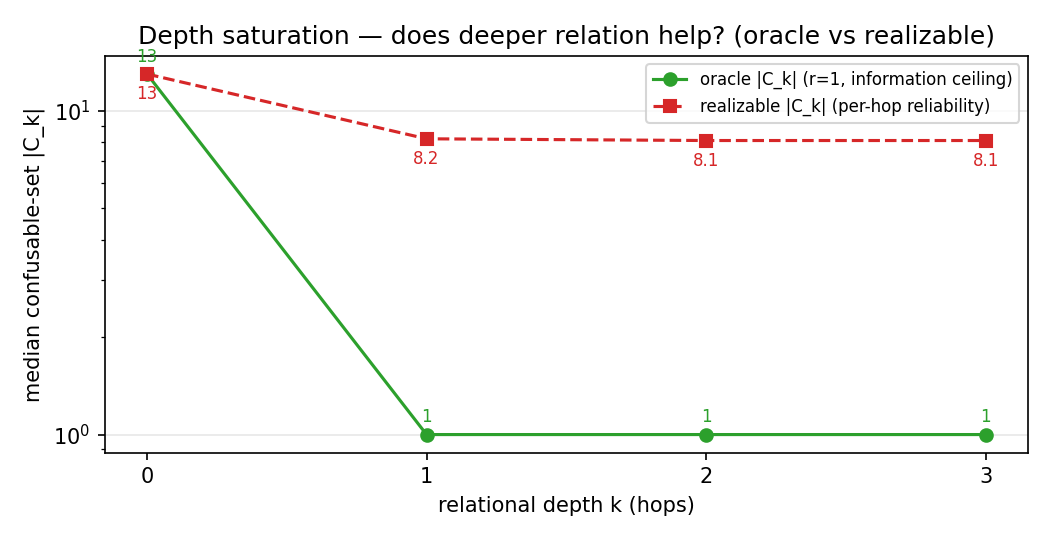
\includegraphics[width=0.85\textwidth]{depth_saturation.png}
  \caption{Information versus realizability. The oracle confusable set keeps shrinking with depth; the
  reliability-weighted realizable set saturates at one hop --- the depth law.}
  \label{fig:depth}
\end{figure}

\subsection{Failure decomposition, latency, and triage effort}
\label{sec:eval-failure}

Because the pipeline localizes errors to named fields rather than opaque scores, the residual
end-to-end loss decomposes cleanly: it is dominated by \emph{extraction} errors --- missing or
incorrect spatial predicates and the lowest-accuracy fields (subtype, material, position-context) ---
not by retrieval logic. Every failure has a traceable stage, which is the operational
differentiator over black-box matching: the roadmap is ``improve the named weak fields,'' not
``redesign the planner.'' Latency favors the constrained pipeline (${\sim}1$\,s vs.\ ${\sim}4.5$\,s
for the ReAct agent, with exact repeatability). The workflow-facing cost metric makes the ceiling
concrete (Figure~\ref{fig:triage}): the expected number of candidates a coordinator must inspect falls
from a median 38 under manual scan to 0.5 under a perfect address --- with 15 seconds per inspection an
explicit proxy assumption, not a user-study result.

\begin{figure}[ht]
  \centering
  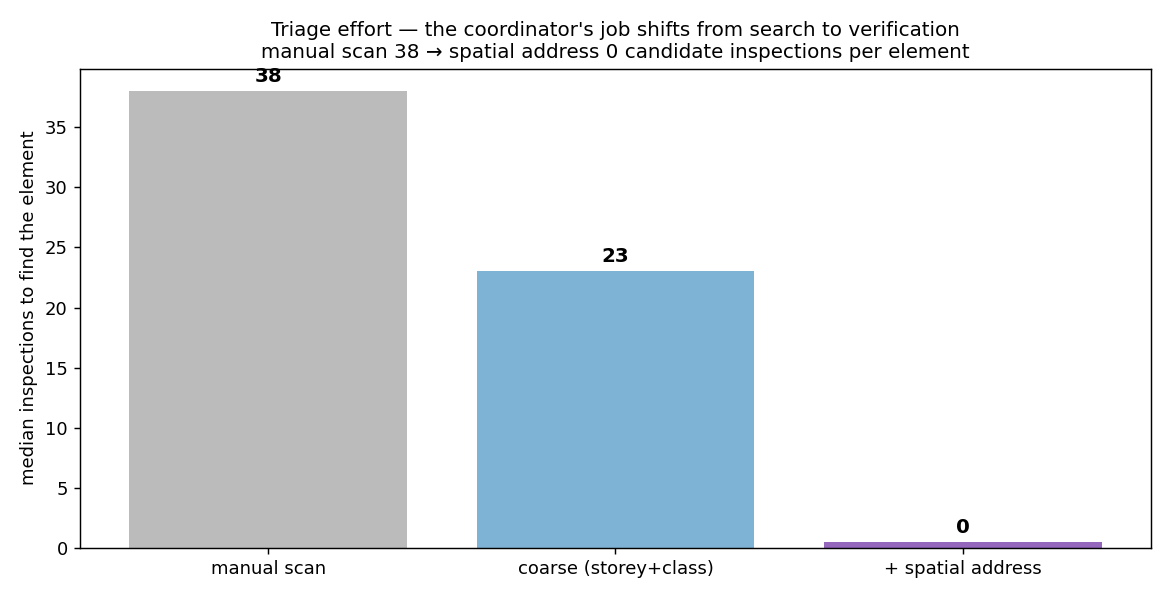
\includegraphics[width=0.8\textwidth]{triage_effort.png}
  \caption{Triage-effort proxy on the same held-out pools. Expected inspections per case fall from a
  median 38 (manual scan) to 0.5 (perfect address); the realized specialist sits between, with
  success@1 78.5\% under the oracle address.}
  \label{fig:triage}
\end{figure}

\section{Discussion}
\label{sec:discussion}

\subsection{Workflow impact: a before/after walkthrough}
\label{sec:workflow}

The system's value is best seen as a concrete walkthrough rather than a claim.

\paragraph{Before (manual workflow).} A site worker photographs a cracked column near a stairwell on
floor 12 and writes a chat message: ``crack near stairs, floor 12, block A.'' The coordinator reads it
at end of day, goes on a site walk, identifies the element by sight, and manually types the IFC GUID
into the issue tracker. Average lag: 1--3 days. If the coordinator leaves the project, the knowledge
leaves with them. The element lands in a flat spreadsheet, not linked to the BIM record, and downstream
compliance requires manual re-entry.

\paragraph{After (system-assisted).} The worker sends the same photo and message. The system returns a
compact ranked shortlist within ${\sim}1$ second --- the pool compressed from ${\sim}1{,}200$ elements
to a median of a few dozen, with the correct element in the pool ${\sim}100\%$ of the time and, on the
addressable subset, at rank 1 in 67.6\% of answered cases (80.6\% when the system is allowed to defer
the least-confident fifth). The worker taps the correct element; a BCF package is generated and the
element is linked to the BIM record. The coordinator's role shifts from data entry to verifying and
escalating a shortlist, and no longer requires being on-site to resolve the link.

The claim is deliberately bounded: this does not replace the coordinator. It eliminates the manual
data-entry loop, surfaces the correct element inside a short ranked shortlist, abstains explicitly
when unsure, and improves over the project lifecycle as confirmed GUIDs accumulate as supervision.

\subsection{Limitations}
\label{sec:limitations}

We state the boundaries directly. \emph{Synthetic-to-real gap (central limitation):} all training and
evaluation data are synthetic; the numbers are optimistic until validated on real site photographs,
and a small pilot (50--100 labelled real cases from a live project) is the single most informative
next measurement. \emph{Single project:} the ceilings and reliabilities are measured on one synthetic
model; the form of the contribution (type-conditional, shallow, image-recoverable, calibrated-soft) is
general, the specific numbers are not. \emph{Statistical power:} the calibration and
coverage--accuracy estimates rest on 35 addressable fillers; we report the operating point (defer
${\sim}20\% \to 80.6\%$), not a precise optimal threshold. \emph{Class coverage:} the realized address
covers fillers; the wall fingerprint is demonstrated at oracle level and is blocked from realization
by the image-recoverability constraint itself (\secref{sec:eval-realized}); ``other''-class and
room-relative addressing remain open. \emph{Multi-hop:} joint multi-hop extraction collapses under
error cascade; practical use is single-hop plus human review, by design. \emph{IFC dependency:} the
system retrieves against the model as given; if the IFC is outdated, retrieval is against stale ground
truth --- mitigated by versioning the graph and surfacing low-confidence results for manual check.

\subsection{Future work, prioritized}
\label{sec:future}

\begin{enumerate}
  \item \textbf{Real project traces.} Validate on live coordination data; the synthetic-to-real shift
  is the most credible threat to the numbers and the first thing to measure.
  \item \textbf{Remaining address classes.} Size-band realization (the ResNet head), relation-direction
  improvement via subtype-contrastive augmentation, and room/space addressing where the export carries
  space boundaries.
  \item \textbf{Learned spatial topology.} Replace the distance-threshold \texttt{ADJACENT\_TO}
  heuristic with a learned spatial graph model to generalize beyond standard geometries.
  \item \textbf{Write-back integration.} BCF and BIM-cloud integration, so the grounded GUID lands in a
  live workflow rather than a report; the human feedback loop then converts confirmed GUIDs into
  supervised updates.
  \item \textbf{4D temporal context.} Schedules, timestamps, and progress updates, making the IFC
  graph a dynamic project database rather than a static snapshot.
\end{enumerate}

The long-term goal is not to replace construction managers but to remove the manual translation
burden between physical on-site evidence and the digital record --- supporting timely, traceable, and
continuously updated project analytics.

\section{Conclusion}
\label{sec:conclusion}

We asked how unstructured, egocentric site evidence can be grounded to a unique element in an
allocentric BIM model, in a cold-start regime with no real labels. The answer is a neuro-symbolic
decomposition organized around an \textbf{ontology-grounded, topology-derived spatial address}. The
oracle analysis proves the architecture sound --- the symbolic layer retains the ground truth in 100\%
of cases and, supplied with the type-conditional address, reorders the pool from Top-1 4.9\% to
78.5\% --- and isolates extraction, not retrieval design, as the bottleneck. The realization study
shows how much of that ceiling survives a real detector and how to consume a noisy address: as a
calibrated soft prior inside a recall-fixed pool (union, never intersection), with one deterministic
specialist lifting the addressable subset from 6.6\% to 67.6\% and selective prediction raising the
answered subset to 80.6\% --- the system knows when to abstain. The depth analysis supplies the
architectural principle both rely on: realizable relational discrimination saturates at one hop, so
depth is compiled into the node and learning is placed at the neural$\to$symbolic interface.

Three findings generalize beyond this system. An address field is deployable only if it is defined in
a frame the evidence carries --- image-recoverability is a design constraint, not an afterthought.
When a mature signal combines with an immature one, union preserves recall and intersection destroys
it. And calibration's payoff here is not reweighting (a measured no-op) but \emph{selective
prediction}: the honest deliverable of a grounding system with downstream consequence is a
coverage--accuracy curve and an explicit defer route. Within the regime we can measure, the structured
spatial address is what makes site-to-BIM grounding realizable, auditable, and transferable; validating
it on real project traces is the immediate next step.


\bibliographystyle{plainnat}
\bibliography{references}

\end{document}
